% =====================================================================
%  Does machine learning improve on simple tools for osteoporosis
%  screening? Temporal validation, calibration and subgroup performance
%  in NHANES.   Build:  tectonic main.tex   (or pdflatex main, twice)
%  Revision 9 (IECV primary estimand; clinical-only model; strata and weighted case counts)
% =====================================================================
\documentclass[11pt,a4paper]{article}

\usepackage[T1]{fontenc}
\usepackage[utf8]{inputenc}
\usepackage{lmodern}
\usepackage[margin=2.5cm]{geometry}
\usepackage{amsmath,amssymb}
\usepackage{graphicx}
\usepackage{booktabs}
\usepackage{array}
\usepackage{longtable}
\usepackage{caption}
\usepackage{float}
\usepackage{enumitem}
\usepackage{setspace}
\usepackage[left]{lineno}
\usepackage{tikz}
\usetikzlibrary{positioning,arrows.meta,calc}
\usepackage[colorlinks=true,linkcolor=blue!50!black,citecolor=blue!50!black,urlcolor=blue!50!black]{hyperref}

\graphicspath{{figures/}}
\captionsetup{font=small,labelfont=bf}
\setlist{nosep,leftmargin=*}
\onehalfspacing
\linenumbers
\emergencystretch=3em

\begin{document}

% ---------------------------------------------------------------- Title page
\begin{titlepage}
\begin{center}
{\LARGE\bfseries Does Machine Learning Improve on Simple Tools for Osteoporosis Screening? Internal--External Validation, Calibration and Subgroup Performance in NHANES\par}
\vspace{1.5em}
{\large Sulaxan Jadhav$^{*}$\par}
\vspace{1em}
{\small Symbiosis School of Economics, Symbiosis International (Deemed University), Pune, India\\[2pt]
ORCID: \href{https://orcid.org/0000-0003-2500-6030}{0000-0003-2500-6030}\\[2pt]
$^{*}$Corresponding author: Dr Sulaxan Jadhav, Symbiosis School of Economics, Symbiosis International (Deemed University), Pune, India. E-mail: \href{mailto:sulaxan.jadhav@sse.ac.in}{sulaxan.jadhav@sse.ac.in}\par}
\end{center}
\vspace{2em}
\noindent\textbf{Running title:} Machine learning vs simple tools for osteoporosis screening\\[4pt]
\textbf{Word count:} 3,160 (main text, excluding abstract, tables, figure legends and references)\\[2pt]
\textbf{Tables:} 5 \quad \textbf{Figures:} 4 (+23 supplementary tables, 2 supplementary figures)\\[4pt]
\textbf{Keywords:} osteoporosis; mass screening; machine learning; Osteoporosis Self-Assessment Tool; internal--external cross-validation; NHANES

\vfill
\noindent\textbf{Statements and Declarations}

\noindent\textbf{Funding.} This research received no specific grant from any funding agency in the public, commercial or not-for-profit sectors.\\
\textbf{Competing interests.} The author declares no competing interests.\\
\textbf{Ethics approval.} NHANES protocols were approved by the NCHS Research Ethics Review Board, and all participants provided written informed consent. This secondary analysis of publicly available, de-identified data did not require additional institutional review.\\
\textbf{Consent to participate.} Written informed consent was obtained by NCHS from all NHANES participants.\\
\textbf{Consent for publication.} Not applicable.\\
\textbf{Data availability.} NHANES data are publicly available from the National Center for Health Statistics (\url{https://www.cdc.gov/nchs/nhanes/}).\\
\textbf{Code availability.} Analysis code, including the fitted model equations, is available at \url{https://github.com/slxnjdhv/osteoporosis-nhanes}.\\
\textbf{Protocol and registration.} No study protocol was prepared in advance and the study was not registered.\\
\textbf{Patient and public involvement.} None.\\
\textbf{Author contributions.} Sulaxan Jadhav: conceptualisation, methodology, software, formal analysis, data curation, visualisation, writing -- original draft, and writing -- review and editing. The author read and approved the final manuscript.\\
\textbf{Use of AI tools.} Claude (Anthropic) was used for analytic and generative tasks, as described in the Methods (Software).
\end{titlepage}


% ---------------------------------------------------------------- Abstract
\begin{abstract}
\noindent\textbf{Background.} Machine learning (ML) models for osteoporosis screening are rarely compared with simple clinical tools under equal conditions.

\noindent\textbf{Methods.} We studied 9,657 adults aged $\ge$50 years in five NHANES cycles (2005--2018), not diagnosed with or treated for osteoporosis; the outcome was a hip T-score $\le -2.5$. Seven model families using 35 clinical, laboratory and socio-demographic predictors were tuned equally and recalibrated. In internal--external cross-validation (IECV) across cycles, logistic regression was compared with the Osteoporosis Self-Assessment Tool (OST), a sex-specific OST, ORAI, SCORE and an age--weight--sex model, and the other families with logistic regression. The main estimand, chosen after earlier analyses (all reported), was the pooled AUROC difference from OST; the equivalence margin was $\pm$0.02. The study is exploratory.

\noindent\textbf{Results.} Penalised logistic regression was not outperformed: in IECV, five of six tuned ML families were equivalent to it, and none was better. In IECV it exceeded OST by 0.024 in AUROC (95\% CI 0.009--0.038) and the age--weight--sex model by 0.019 (0.004--0.033); their clinical relevance was uncertain. A clinical model without blood tests, race or income exceeded OST by 0.016 (0.004--0.029). Referring 20\% of people for DXA, the full model detected 2.8 (1.0--4.3) more cases per 1,000 screened than OST (8.6\% more), and the clinical model 1.7 more.

\noindent\textbf{Conclusions.} Equally tuned ML did not outperform logistic regression. Thirty-five predictors gave a small, consistent gain over simple tools, about three cases per 1,000 screened at equal DXA capacity; whether that justifies a complex tool is a local judgement.
\end{abstract}

% ================================================================= 1 Introduction
\section{Introduction}

Osteoporosis causes fragility fractures that lead to disability, loss of independence and excess mortality, yet effective treatment substantially lowers fracture risk once the disease is recognised \cite{compston2019}. Among US adults aged 50 years and older, about one in eight has osteoporosis at the femoral neck or lumbar spine \cite{sarafrazi2021}. Diagnosis relies on dual-energy X-ray absorptiometry (DXA), with osteoporosis defined as a T-score of $-2.5$ or lower \cite{kanis1994}. DXA capacity is limited, and guidelines target screening mainly at women aged 65 and older and at younger postmenopausal women at increased risk, leaving men and many younger women under-assessed \cite{uspstf2025}.

Simple risk tools can prioritise who most needs DXA. The Osteoporosis Self-Assessment Tool (OST), $0.2\times(\text{weight}-\text{age})$, uses only age and weight \cite{geusens2002,koh2001}; the Osteoporosis Risk Assessment Instrument (ORAI) and the Simple Calculated Osteoporosis Risk Estimation (SCORE) add a few questionnaire items \cite{cadarette2000,lydick1998}. In women these tools reach areas under the receiver operating characteristic curve (AUROC) of about 0.70--0.80 \cite{geusens2002,rud2007,gourlay2008}, systematic reviews have found that further risk factors rarely improve on age and weight \cite{rubin2013,nayak2015}, and OST also performs reasonably in men \cite{adler2003,lynn2008,diem2017}, although its accuracy varies with ethnicity \cite{cass2006}. FRAX calculated without bone mineral density (BMD) identifies low bone density less well than OST \cite{crandall2014,diem2017}, so it is not the natural comparator for a tool that selects people for DXA.

Machine learning (ML) models built on population surveys have reported AUROCs of 0.69--0.74 in the Korea National Health and Nutrition Examination Survey (KNHANES), against 0.73 for logistic regression \cite{shim2020,suh2023}, and of 0.81--0.85 in the US National Health and Nutrition Examination Survey (NHANES) \cite{tang2023,zhangy2025,zhang2025}, where one gradient-boosting model was compared with OST (0.83 vs 0.78) \cite{zhangy2025}. These studies used random splits from the same years, comparators that were absent or tuned less carefully than the ML models, accuracy as the main metric, and cohorts that included people already diagnosed or treated, with little attention to calibration or to men. Across clinical prediction tasks, ML has rarely outperformed logistic regression \cite{christodoulou2019}, and class-imbalance corrections can distort calibration \cite{vandengoorbergh2022}.

We aimed not to propose another model but to estimate how much ML and additional predictors add to simple tools for osteoporosis case-finding in adults neither diagnosed with nor treated for osteoporosis, when every method is tuned equally. We compared equally tuned model families with logistic regression, and logistic regression with OST, a sex-specific OST, ORAI, SCORE and an age--weight--sex model, by internal--external cross-validation across five survey cycles with all tuning nested, and expressed gains as cases detected per 1,000 people screened at a fixed DXA capacity. The study is reported according to TRIPOD+AI \cite{collins2024} (Supplementary Table~\ref{tab:tripod}).

% ================================================================= 2 Methods
\section{Methods}

\subsection{Data source and study population}
We used publicly available, de-identified data from NHANES, a cross-sectional survey of the non-institutionalised US civilian population with a complex, multistage probability design \cite{johnson2013,johnson2014}. We pooled the five 2-year cycles with femoral DXA: 2005--2006, 2007--2008, 2009--2010, 2013--2014 and 2017--2018, merging demographic, body-measure, DXA, laboratory, questionnaire and prescription-medication files on the respondent sequence number.

Of 50,463 participants, 14,166 were aged 50 years or older and 10,981 of these had a valid femoral neck BMD measurement. Because the intended use is case-finding before DXA, we excluded 1,324 participants who reported a physician diagnosis of osteoporosis (1,155) or current use of an osteoporosis medication without such a diagnosis (169); 282 of them met the outcome definition. The final cohort comprised 9,657 participants (Figure~\ref{fig:flow}). No participant missed more than 50\% of predictors. Participants without DXA are compared with the cohort in Supplementary Table~\ref{tab:excl}, and the medication list is given in the Supplementary Methods.

\subsection{Outcome}
The outcome was osteoporosis at the hip, a T-score of $-2.5$ or lower at the femoral neck or total hip \cite{kanis1994}, calculated from the NHANES III reference values for non-Hispanic white women aged 20--29 years \cite{looker1998} for both sexes, as recommended by the International Society for Clinical Densitometry \cite{watts2013}. DXA was performed by trained technologists following the NHANES protocol, independently of the predictors.

The outcome was revised during the analysis from the femoral neck or lumbar spine to the hip, because the share of partial spine scans rose from 15.3\% in 2005--2006 to 38.1\% in 2017--2018. Every version of the analysis is reported in Supplementary Table~\ref{tab:versions}, and two spine-inclusive outcomes were analysed as sensitivity analyses \cite{baim2008,wright2014}.

Hip DXA used Hologic QDR-4500A densitometers up to 2009--2010 and Hologic Discovery densitometers thereafter, without a published hip cross-calibration. Mean femoral neck BMD in women was about 0.15 reference SD lower from 2013, whereas hip-based prevalence was stable (4.0\%--4.8\% by cycle), so we repeated the analysis with the T-scores of either scanner period shifted by 0.15 SD.

\subsection{Predictors and data preparation}
We considered 35 candidate predictors (32 variables, with race/ethnicity entered as four indicators) obtainable from history, examination or standard blood tests: age, sex, race/ethnicity (five categories), education and family income-to-poverty ratio (PIR); body mass index (BMI), weight, height and waist circumference; ten serum measurements (calcium, phosphorus, alkaline phosphatase, creatinine, albumin, uric acid, glucose, total protein, cholesterol and 25-hydroxyvitamin D); FRAX-type risk factors (prior hip, wrist or spine fracture, parental hip fracture, ever daily glucocorticoid use, current smoking, alcohol $\ge$3 drinks/day); and former smoking, postmenopausal status, ever use of female hormones, diabetes, arthritis, coronary heart disease, stroke and cancer. DXA-derived variables and self-reported osteoporosis were excluded to prevent leakage. Non-Hispanic Asian adults can be identified only from 2011, so in the models they fall within ``other/multiracial''; this category made up 2.9\%--4.6\% of participants in 2005--2010 and 17.8\% in 2017--2018.

Age (top-coded differently by cycle), creatinine (2005--2006 method change), vitamin D and alcohol (questionnaire change in 2017--2018) were harmonised across cycles as described in the Supplementary Methods. Reproductive variables were coded 0 for men. Missingness by cycle is shown in Supplementary Table~\ref{tab:miss}.

\subsection{Development set and missing data}
Participants from 2005--2014 ($n=7{,}649$; 343 cases) formed the development set for model selection, and those from 2017--2018 ($n=2{,}008$; 96 cases) the temporal validation set, which had been evaluated in earlier versions of the analysis (Supplementary Table~\ref{tab:versions}). With 9.8 events per candidate predictor, all regression models were penalised. Missing predictor values (at most 9.5\% overall and 14.6\% in any cycle; Supplementary Table~\ref{tab:miss}) were imputed once by chained equations \cite{vanbuuren2011}, fitted within each training fold without the outcome; binary predictors were not rounded.


\subsection{Models and tuning}
We compared eight model families: ridge-penalised logistic regression (LR); LR with cubic B-splines for the 17 continuous or ordinal predictors (LR-spline) \cite{perperoglou2019}; a support vector machine (SVM); random forest (RF); XGBoost \cite{chen2016}, LightGBM \cite{ke2017} and CatBoost \cite{prokhorenkova2018}; and a stacking ensemble of the four tree-based models. Each was fitted with three class-imbalance strategies (none, class weighting and SMOTE \cite{chawla2002}), and the seven single learners were tuned with their best strategy by Bayesian optimisation (Optuna \cite{akiba2019}; 40 trials each) in 5-fold cross-validation (Supplementary Table~\ref{tab:hyper}; Supplementary Figure~\ref{fig:workflow}). The family with the highest tuned cross-validated AUROC was selected as the full model.

\subsection{Benchmarks}
Comparators were OST \cite{geusens2002}, without fitting, including at its usual cut-offs ($<2$ and $<-1$) \cite{rud2007}; a sex-specific OST (a logistic model of OST, sex and their interaction); ORAI \cite{cadarette2000} and SCORE \cite{lydick1998}, adapted to the available items (Supplementary Methods); LR with age, weight and sex; and a Boruta + XGBoost pipeline following Zhang et al.\ \cite{zhang2025,kursa2010}. For calibration and net benefit, the scores were converted to probabilities by logistic recalibration. We also fitted the full model without race/ethnicity \cite{vyas2020}; without race/ethnicity, income and education (clinical + laboratory); and without laboratory tests as well (clinical: 19 history and examination items). Several clinical items (parental hip fracture, glucocorticoid use, alcohol) are often missing or unreliable in routine records, so the clinical model approximates, but does not test, a tool based on electronic health records.

\subsection{Recalibration, thresholds and performance measures}
Every model was recalibrated by Platt scaling \cite{platt2000} on its out-of-fold development predictions. We assessed discrimination (AUROC and area under the precision--recall curve, AUPRC), calibration (slope, calibration-in-the-large and Brier score) \cite{vancalster2019} and net benefit at thresholds of 2\%--15\% \cite{vickers2006}, with the development-set Youden threshold \cite{youden1950} as the primary operating point. Because AUROC differences are hard to interpret clinically \cite{dehond2022}, we also counted cases detected per 1,000 people screened when 15\%, 20\%, 25\% or 30\% of people, ranked by each tool, were referred for DXA.


\subsection{Estimands and tests}
The main estimand was the pooled IECV difference in AUROC between the full model and OST. With an equivalence margin of $\pm$0.02, a gain was classified as \emph{relevant} if its lower 95\% limit exceeded 0.02, \emph{superior but of uncertain relevance} if its 95\% CI excluded zero but included 0.02, and \emph{equivalent} if its 90\% CI lay within $\pm$0.02 (two one-sided tests); the same rule was applied to each ML family versus LR, without multiplicity adjustment. The estimand and margin were chosen after earlier versions of the analysis had seen the data, so the study is exploratory and its $P$ values are descriptive. For the 2017--2018 split we also report the post hoc hierarchy of earlier versions: the full model versus OST, then versus ORAI, SCORE, the three-variable model and Boruta + XGBoost with Holm adjustment \cite{holm1979}.

\subsection{Internal--external validation and model-fitting uncertainty}
Each of the five cycles was held out in turn \cite{steyerberg2016}, and every model was developed on the other four. The LR penalties were re-tuned there (40 Optuna trials), except for the three-variable model (fixed $C=1$), and each ML family re-selected its imbalance strategy and was re-tuned in the same way, so that no held-out cycle informed any model choice; stacking was omitted for run time. AUROC differences within each cycle were estimated by paired bootstrap and pooled by DerSimonian--Laird random effects \cite{dersimonian1986} with Hartung--Knapp--Sidik--Jonkman (HKSJ) CIs \cite{inthout2014}, whose variance was not allowed below the DerSimonian--Laird variance, and 95\% prediction intervals; single AUROCs were pooled with Hanley--McNeil standard errors \cite{hanley1982}. Because the development sets overlap, these CIs are approximate; as a check, we also bootstrapped the pooled out-of-cycle predictions within cycles. Cases per 1,000 were computed on the pooled out-of-cycle predictions, with referral applied within each cycle, ties broken at random and bootstrap CIs conditional on the fitted models: overall, in the population not routinely screened (everyone except women aged 65 or older; evidence for screening men is insufficient \cite{uspstf2025}), in guideline strata and with survey weights. In the 2017--2018 split, CIs came from 1,000 paired bootstrap resamples, and a refit bootstrap (1,000 replicates) also resampled the development set and refitted the models.

\subsection{Survey weighting and non-response}
Models were fitted without survey weights. Pooled descriptive estimates used the examination weights divided by five. For 2017--2018 we also estimated weighted performance with design-based CIs (Rao--Wu bootstrap, 500 replicates) \cite{chen2020,raowu1988} and, because 22.5\% of eligible participants lacked valid DXA, with weights adjusted for non-response by the inverse probability of having DXA (modelled from age, sex, education, PIR, BMI, race/ethnicity and cycle), trimmed or capped in sensitivity analyses \cite{potter1990,lee2011}.

\subsection{Subgroups, clinical strata and sensitivity analyses}
In 2017--2018 we evaluated performance by sex, age and race/ethnicity (reporting non-Hispanic Asian adults separately), in four guideline strata (women aged 50--64 and $\ge$65 years, men aged 50--69 and $\ge$70 years) \cite{uspstf2025}, and with sex-specific thresholds. Sensitivity analyses used spine-inclusive outcomes, included diagnosed or treated participants, shifted T-scores, excluded non-Hispanic Asian participants, developed on 2013--2014 alone or without 2005--2006, and omitted laboratory predictors or alcohol. Predictor importance (SHAP) \cite{lundberg2017} and a re-implementation of a published pipeline are reported in the Supplement.

\subsection{Software}
Analyses used Python 3.9.6 with scikit-learn 1.6.1 \cite{pedregosa2011}, XGBoost 2.1.4, LightGBM 4.6.0, CatBoost 1.2.10, Optuna 5.0.0, SHAP 0.49.1 and statsmodels 0.14.6 (full list in the code repository), with a fixed random seed. Two-sided $P<0.05$ was considered significant. A large language model, Claude (Anthropic; Claude Opus models, most recently Claude Opus 5.5, accessed through the Claude Code desktop application in 2026), was used to write and run the analysis code, to draft and revise the manuscript text and tables, and to carry out independent critical reviews of drafts, in response to the author's instructions (representative prompts: ``run internal--external cross-validation with the tuning nested in each development set; ``review the manuscript as a journal referee and check every number against the outputs). Every reported number is generated by the public code from public data, and each analysis version is listed in Supplementary Table~\ref{tab:versions}; the author is responsible for the content.

% -------- Figure 1: participant flow
\begin{figure}[!htbp]
\centering
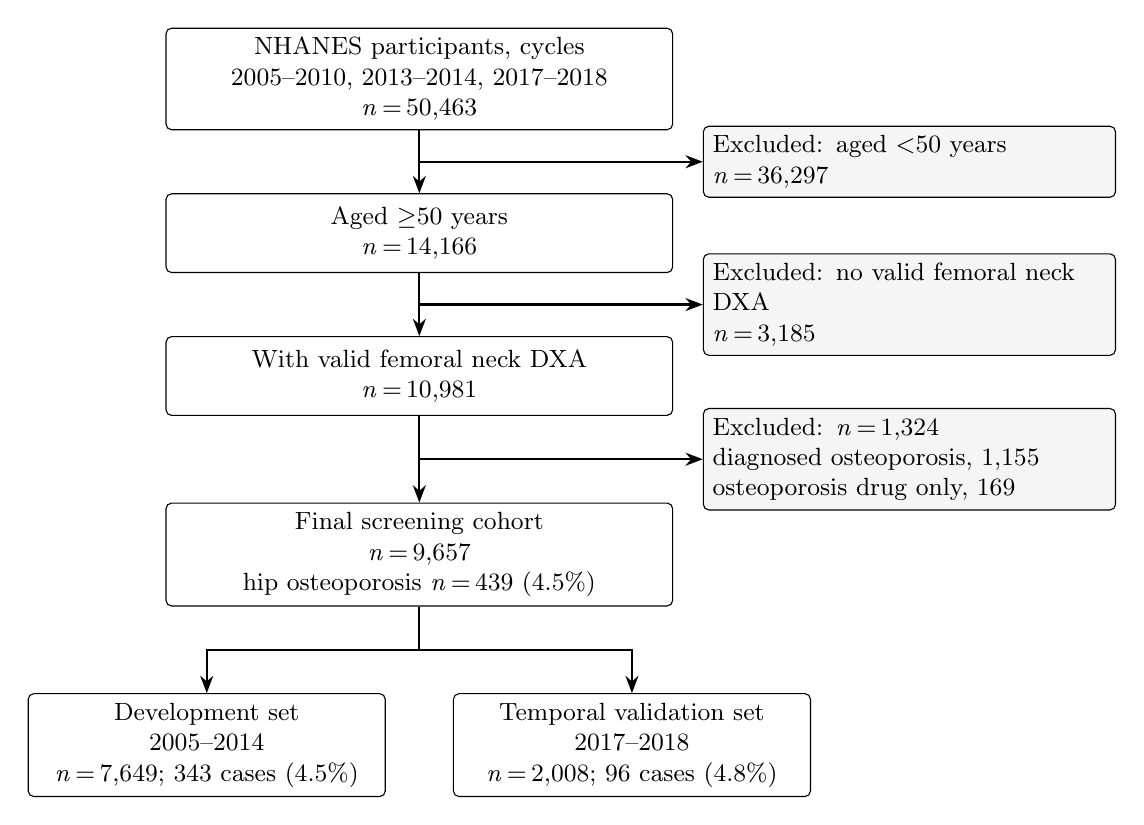
\begin{tikzpicture}[
  box/.style={draw, rounded corners=2pt, align=center, text width=6.2cm, minimum height=1cm, font=\small},
  ex/.style={draw, rounded corners=2pt, align=left, text width=5.0cm, font=\small, fill=gray!8},
  arr/.style={-{Stealth[length=2.2mm]}, thick},
  node distance=0.8cm]
\node[box] (a) {NHANES participants, cycles 2005--2010, 2013--2014, 2017--2018\\ \textit{n}\,=\,50,463};
\node[box, below=of a] (b) {Aged $\ge$50 years\\ \textit{n}\,=\,14,166};
\node[box, below=of b] (b2) {With valid femoral neck DXA\\ \textit{n}\,=\,10,981};
\node[box, below=1.1cm of b2] (c) {Final screening cohort\\ \textit{n}\,=\,9,657\\ hip osteoporosis \textit{n}\,=\,439 (4.5\%)};
\coordinate (m1) at ($(a.south)!0.5!(b.north)$);
\coordinate (m2) at ($(b.south)!0.5!(b2.north)$);
\coordinate (m3) at ($(b2.south)!0.5!(c.north)$);
\node[ex, anchor=west] (x1) at ($(m1)+(3.6,0)$) {Excluded: aged $<$50 years\\ \textit{n}\,=\,36,297};
\node[ex, anchor=west] (x2) at ($(m2)+(3.6,0)$) {Excluded: no valid femoral neck DXA\\ \textit{n}\,=\,3,185};
\node[ex, anchor=west] (x3) at ($(m3)+(3.6,0)$) {Excluded: \textit{n}\,=\,1,324\\ diagnosed osteoporosis, 1,155\\ osteoporosis drug only, 169};
\node[box, text width=4.3cm, anchor=north] (d) at ($(c.south)+(-2.7,-1.1)$) {Development set\\ 2005--2014\\ \textit{n}\,=\,7,649; 343 cases (4.5\%)};
\node[box, text width=4.3cm, anchor=north] (e) at ($(c.south)+(2.7,-1.1)$) {Temporal validation set\\ 2017--2018\\ \textit{n}\,=\,2,008; 96 cases (4.8\%)};
\draw[arr] (a) -- (b); \draw[arr] (b) -- (b2); \draw[arr] (b2) -- (c);
\draw[arr] (m1) -- (x1.west);
\draw[arr] (m2) -- (x2.west);
\draw[arr] (m3) -- (x3.west);
\draw[thick] (c.south) -- ++(0,-0.55) coordinate (split);
\draw[arr] (split) -| (d.north);
\draw[arr] (split) -| (e.north);
\end{tikzpicture}
\caption{Participant flow. Percentages are the prevalence of osteoporosis at the hip (femoral neck or total hip T-score $\le -2.5$). No participant was excluded for missing more than 50\% of predictors.}
\label{fig:flow}
\end{figure}


% ================================================================= 3 Results
\section{Results}

\subsection{Participants}
The cohort comprised 9,657 adults (mean age 64.2 years; 43.0\% women), of whom 439 (4.5\%; survey-weighted 3.9\%) had undiagnosed hip osteoporosis, 4.0\%--4.8\% by cycle. Participants with osteoporosis were older, more often women, smaller and poorer, and more often had a prior fracture (22.3\% vs 11.6\%) (Table~\ref{tab:baseline}). The 2017--2018 cycle had more participants of other or multiracial ethnicity (17.8\% vs 5.9\%) and differed in several laboratory values (Supplementary Table~\ref{tab:devval}).

\begin{table}[!htbp]
\centering
\caption{Baseline characteristics by osteoporosis status ($n=9{,}657$). Values are mean (SD) or $n$ (\%); weighted columns are survey-weighted means or percentages. $P$ values are from unweighted Welch's $t$-tests or $\chi^2$ tests. Percentages are of participants with a non-missing value; reproductive variables were coded 0 for men, so their percentages include men in the denominator.}
\label{tab:baseline}
\footnotesize
\setlength{\tabcolsep}{4pt}
\begin{tabular}{lccccc}
\toprule
 & \multicolumn{2}{c}{Unweighted} & & \multicolumn{2}{c}{Weighted} \\
\cmidrule{2-3}\cmidrule{5-6}
Characteristic & No ($n=9{,}218$) & Yes ($n=439$) & $P$ & No & Yes \\
\midrule
Age, years & 63.88 (9.25) & 71.14 (9.07) & $<$0.001 & 61.9 & 70.0 \\
Female sex & 3,833 (41.6) & 318 (72.4) & $<$0.001 & 45.3 & 76.5 \\
Postmenopausal & 3,351 (37.1) & 293 (70.4) & $<$0.001 & 39.7 & 74.7 \\
Ever used female hormones & 1,299 (14.4) & 70 (16.9) & 0.18 & 17.8 & 19.5 \\
Prior hip, wrist or spine fracture & 1,069 (11.6) & 98 (22.3) & $<$0.001 & 13.4 & 23.4 \\
Parental hip fracture & 889 (9.9) & 45 (10.7) & 0.65 & 11.1 & 12.5 \\
Ever daily glucocorticoid use & 495 (5.4) & 22 (5.1) & 0.85 & 6.1 & 7.3 \\
Alcohol $\ge$3 drinks/day & 222 (2.5) & 3 (0.7) & 0.036 & 2.5 & 1.3 \\
Current smoker & 1,562 (17.0) & 92 (21.0) & 0.035 & 15.6 & 25.3 \\
Stroke & 512 (5.6) & 45 (10.3) & $<$0.001 & 4.4 & 8.4 \\
Diabetes & 1,771 (19.2) & 77 (17.5) & 0.42 & 14.7 & 12.3 \\
Non-Hispanic Black & 1,991 (21.6) & 43 (9.8) & $<$0.001 & 9.7 & 4.6 \\
Income-to-poverty ratio & 2.74 (1.62) & 2.10 (1.37) & $<$0.001 & 3.33 & 2.43 \\
BMI, kg/m$^2$ & 28.94 (5.53) & 24.41 (4.46) & $<$0.001 & 28.97 & 24.37 \\
Weight, kg & 81.51 (17.75) & 62.23 (13.56) & $<$0.001 & 82.8 & 62.4 \\
Height, cm & 167.67 (9.84) & 159.44 (8.93) & $<$0.001 & 168.8 & 159.9 \\
Waist, cm & 101.60 (13.62) & 90.73 (13.29) & $<$0.001 & 101.7 & 90.0 \\
Alkaline phosphatase, U/L & 74.31 (24.62) & 82.85 (28.38) & $<$0.001 & 71.9 & 82.5 \\
Uric acid, mg/dL & 5.72 (1.43) & 5.29 (1.44) & $<$0.001 & 5.62 & 5.12 \\
25(OH) vitamin D, nmol/L & 67.37 (27.85) & 67.17 (30.44) & 0.90 & 72.8 & 69.3 \\
\bottomrule
\end{tabular}
\end{table}


\subsection{Model selection}
With default hyperparameters and each family's best imbalance strategy, cross-validated AUROC ranged from 0.841 (SVM) to 0.876 (LR); after equal tuning, seven of eight families lay within 0.006 of each other (0.873--0.879; RF 0.864) (Supplementary Table~\ref{tab:tuned}). LR remained the highest (0.879) and was selected as the full model. Tuned XGBoost and LightGBM converged on stumps, that is, on additive models. Class weighting and SMOTE raised the raw Brier score of LR from 0.035 to 0.127--0.137, which recalibration removed.

\subsection{Internal--external validation across cycles}
The full model exceeded OST and the three-variable model in every held-out cycle (Table~\ref{tab:iecv}). The pooled gain was 0.024 (95\% HKSJ CI 0.009--0.038; prediction interval 0.007--0.040) over OST and 0.019 (0.004--0.033) over the three-variable model ($I^2$ 0\% and 29\%): better than both, but of uncertain relevance, since the CIs span 0.02. Pooling the out-of-cycle predictions instead gave 0.026 (0.015--0.036) over OST. The gain over the sex-specific OST was 0.017 (0.004--0.029). Most of the gain remained without race/ethnicity (0.021, 0.007--0.034, over OST) and without race, income and education (0.020, 0.007--0.033). The clinical model, which also omits blood tests, had a pooled AUROC of 0.871 and exceeded OST by 0.016 (0.004--0.029) and the three-variable model by 0.011 ($-$0.005 to 0.027); the full model exceeded it by 0.011 (0.003--0.019) (Supplementary Table~\ref{tab:iecvclin}). Across cycles, the full model's AUROC ranged from 0.841 to 0.912, its calibration slope from 0.82 to 1.25 and its observed-to-expected ratio from 0.84 to 1.16. The tuned penalty was stable ($C$ = 0.13--0.94) except when 2005--2006 was held out ($C$ = 22.5), and re-tuning changed the pooled AUROC by only 0.001.

With every ML family re-tuned inside each development set, SVM, LR-spline, XGBoost, LightGBM and CatBoost were equivalent to the full model (pooled differences $-$0.006 to $-$0.002; 90\% CIs within $-$0.012 to 0.005), none was better, and RF was not shown to be equivalent ($-$0.010; 90\% CI $-$0.021 to 0.000) (Supplementary Table~\ref{tab:iecvml}).

\begin{table}[!htbp]
\centering
\caption{Internal--external cross-validation: each cycle held out in turn, with models developed on the other four cycles and the penalty of each regression model except the three-variable model (fixed $C=1$) re-tuned within the development cycles (40 Optuna trials). $\Delta$, full model minus comparator (paired bootstrap within the held-out cycle; 95\% CI as difference $\pm$1.96 bootstrap SD). Pooled estimates from a DerSimonian--Laird random-effects model with Hartung--Knapp--Sidik--Jonkman (HKSJ) 95\% CIs; single AUROCs pooled with Hanley--McNeil standard errors. O/E, observed to expected cases. R/S-free, full model without race/ethnicity, income and education; AWS, age--weight--sex model; OST-sex, sex-specific OST.}
\label{tab:iecv}
\footnotesize
\setlength{\tabcolsep}{2pt}
\resizebox{\textwidth}{!}{%
\begin{tabular}{lrrcccccccc}
\toprule
 & & & \multicolumn{5}{c}{AUROC} & & & \\
\cmidrule(lr){4-8}
Held-out cycle & $n$ & Cases & Full & R/S-free & AWS & OST-sex & OST & $\Delta$ vs OST (95\% CI) & $\Delta$ vs AWS (95\% CI) & Slope; O/E \\
\midrule
2005--2006 & 1,422 & 65 & 0.912 & 0.906 & 0.910 & 0.909 & 0.900 & 0.012 ($-$0.011 to 0.036) & 0.002 ($-$0.014 to 0.019) & 1.09; 0.88 \\
2007--2008 & 2,090 & 84 & 0.901 & 0.902 & 0.873 & 0.873 & 0.867 & 0.034 (0.009--0.058) & 0.028 (0.006--0.050) & 1.25; 0.84 \\
2009--2010 & 2,164 & 100 & 0.877 & 0.874 & 0.853 & 0.858 & 0.858 & 0.019 (0.002--0.036) & 0.024 (0.007--0.041) & 0.93; 1.08 \\
2013--2014 & 1,973 & 94 & 0.841 & 0.828 & 0.811 & 0.813 & 0.808 & 0.033 (0.004--0.062) & 0.030 (0.004--0.056) & 0.82; 1.16 \\
2017--2018 & 2,008 & 96 & 0.869 & 0.863 & 0.851 & 0.850 & 0.841 & 0.028 (0.005--0.051) & 0.018 ($-$0.003 to 0.038) & 1.00; 1.07 \\
\midrule
Pooled & 9,657 & 439 & 0.881 & 0.876 & 0.861 & 0.862 & 0.856 & 0.024 (0.009--0.038) & 0.019 (0.004--0.033) & \\
95\% CI & & & 0.847--0.915 & 0.837--0.914 & 0.817--0.905 & 0.819--0.905 & 0.815--0.897 & & & \\
90\% CI ($\pm$0.02) & & & & & & & & 0.013--0.035 & 0.007--0.030 & \\
\bottomrule
\end{tabular}}
\end{table}


\subsection{Temporal validation}
In 2017--2018, the last fold, the full model's AUROC was 0.869 (0.831--0.904), with a calibration slope of 1.00 (0.85--1.18) (Table~\ref{tab:perf}, Figure~\ref{fig:roc}). It exceeded OST (0.841) by 0.028 (0.007--0.052; $P=0.014$); with the development set also resampled and the models refitted, the CI was $-$0.003 to 0.052. After Holm adjustment it exceeded ORAI (0.791; $P_{\text{Holm}}=0.004$) but not SCORE (0.841; $P_{\text{Holm}}=0.084$), the three-variable model (0.851; $P_{\text{Holm}}=0.14$) or Boruta + XGBoost (0.856; $P_{\text{Holm}}=0.18$). Six of seven tuned ML families (AUROC 0.862--0.872) were equivalent to LR; for RF the upper 90\% limit (0.0204) just exceeded the margin. The sex-specific OST raised OST's AUROC to 0.850 (difference 0.009, 0.002--0.017) by placing men and women on a common risk scale (Supplementary Table~\ref{tab:ostsexspec}). In nested models, body measures, income and education added 0.007 to age, weight and sex, FRAX-type risk factors and history 0.001, laboratory tests 0.005 and race/ethnicity 0.006 (Supplementary Table~\ref{tab:incr}).






\begin{table}[!htbp]
\centering
\caption{Temporal validation performance ($n=2{,}008$; 96 with osteoporosis), with 95\% bootstrap CIs. For OST, ORAI and SCORE, Brier score and slope are for the recalibrated score. $\Delta$AUROC, full model minus each alternative (paired bootstrap; 95\% percentile CI, except 90\% CI for the equivalence family); $P$, two-sided bootstrap $P$; $P_{\text{Holm}}$, Holm-adjusted within its family; not shown for the equivalence family, whose conclusion rests on the 90\% CI. The hierarchy was defined post hoc. Sensitivity, specificity and referrals of every model are in Supplementary Table~\ref{tab:perffull}.}
\label{tab:perf}
\footnotesize
\setlength{\tabcolsep}{3pt}
\resizebox{\textwidth}{!}{%
\begin{tabular}{lccccccc}
\toprule
Model & AUROC (95\% CI) & AUPRC & Brier & Slope (95\% CI) & $\Delta$AUROC (95\% CI) & $P$ & $P_{\text{Holm}}$ \\
\midrule
\textbf{Full model (LR, 35 predictors)} & \textbf{0.869 (0.831--0.904)} & \textbf{0.335} & \textbf{0.038} & \textbf{1.00 (0.85--1.18)} & -- & -- & -- \\
\addlinespace\multicolumn{8}{l}{\textit{Primary comparison}} \\
OST & 0.841 (0.796--0.883) & 0.280 & 0.040 & 0.98 (0.79--1.20) & 0.028 (0.007--0.052) & 0.014 & -- \\
\addlinespace\multicolumn{8}{l}{\textit{Secondary comparisons (Holm-adjusted, family of four)}} \\
LR: age, weight, sex & 0.851 (0.808--0.890) & 0.312 & 0.039 & 1.04 (0.86--1.28) & 0.018 ($-$0.001 to 0.039) & 0.070 & 0.14 \\
SCORE & 0.841 (0.799--0.879) & 0.263 & 0.040 & 1.04 (0.87--1.25) & 0.029 (0.003--0.055) & 0.028 & 0.084 \\
ORAI & 0.791 (0.742--0.834) & 0.177 & 0.042 & 0.93 (0.75--1.11) & 0.078 (0.047--0.115) & 0.001 & 0.004 \\
Boruta + XGBoost pipeline & 0.856 (0.820--0.892) & 0.295 & 0.039 & 1.04 (0.89--1.24) & 0.013 ($-$0.007 to 0.030) & 0.18 & 0.18 \\
\addlinespace\multicolumn{8}{l}{\textit{Tuned ML families vs LR: equivalence (90\% CI, margin $\pm$0.02)}} \\
LR-spline & 0.869 (0.832--0.903) & 0.320 & 0.038 & 1.06 (0.91--1.25) & 0.000 ($-$0.008 to 0.007) & 0.94 & -- \\
SVM & 0.870 (0.832--0.906) & 0.367 & 0.037 & 1.03 (0.87--1.22) & $-$0.001 ($-$0.010 to 0.009) & 0.87 & -- \\
Random forest & 0.862 (0.823--0.900) & 0.313 & 0.038 & 1.04 (0.87--1.24) & 0.007 ($-$0.008 to 0.020) & 0.40 & -- \\
XGBoost & 0.868 (0.834--0.901) & 0.320 & 0.038 & 1.04 (0.90--1.22) & 0.001 ($-$0.010 to 0.012) & 0.88 & -- \\
LightGBM & 0.867 (0.832--0.902) & 0.325 & 0.038 & 1.06 (0.92--1.26) & 0.002 ($-$0.010 to 0.012) & 0.83 & -- \\
CatBoost & 0.867 (0.830--0.905) & 0.333 & 0.038 & 1.07 (0.92--1.26) & 0.002 ($-$0.011 to 0.013) & 0.86 & -- \\
Stacking & 0.872 (0.836--0.908) & 0.338 & 0.038 & 1.04 (0.89--1.24) & $-$0.003 ($-$0.012 to 0.006) & 0.51 & -- \\
\addlinespace\multicolumn{8}{l}{\textit{Exploratory}} \\
OST, sex-specific & 0.850 (0.806--0.890) & -- & -- & -- & 0.019 ($-$0.0004 to 0.041) & 0.060 & -- \\
Full model without race & 0.863 (0.825--0.898) & 0.325 & 0.038 & 1.00 (0.84--1.19) & 0.006 ($-$0.001 to 0.012) & 0.14 & -- \\
\bottomrule
\end{tabular}}
\end{table}

\begin{figure}[!htbp]
\centering
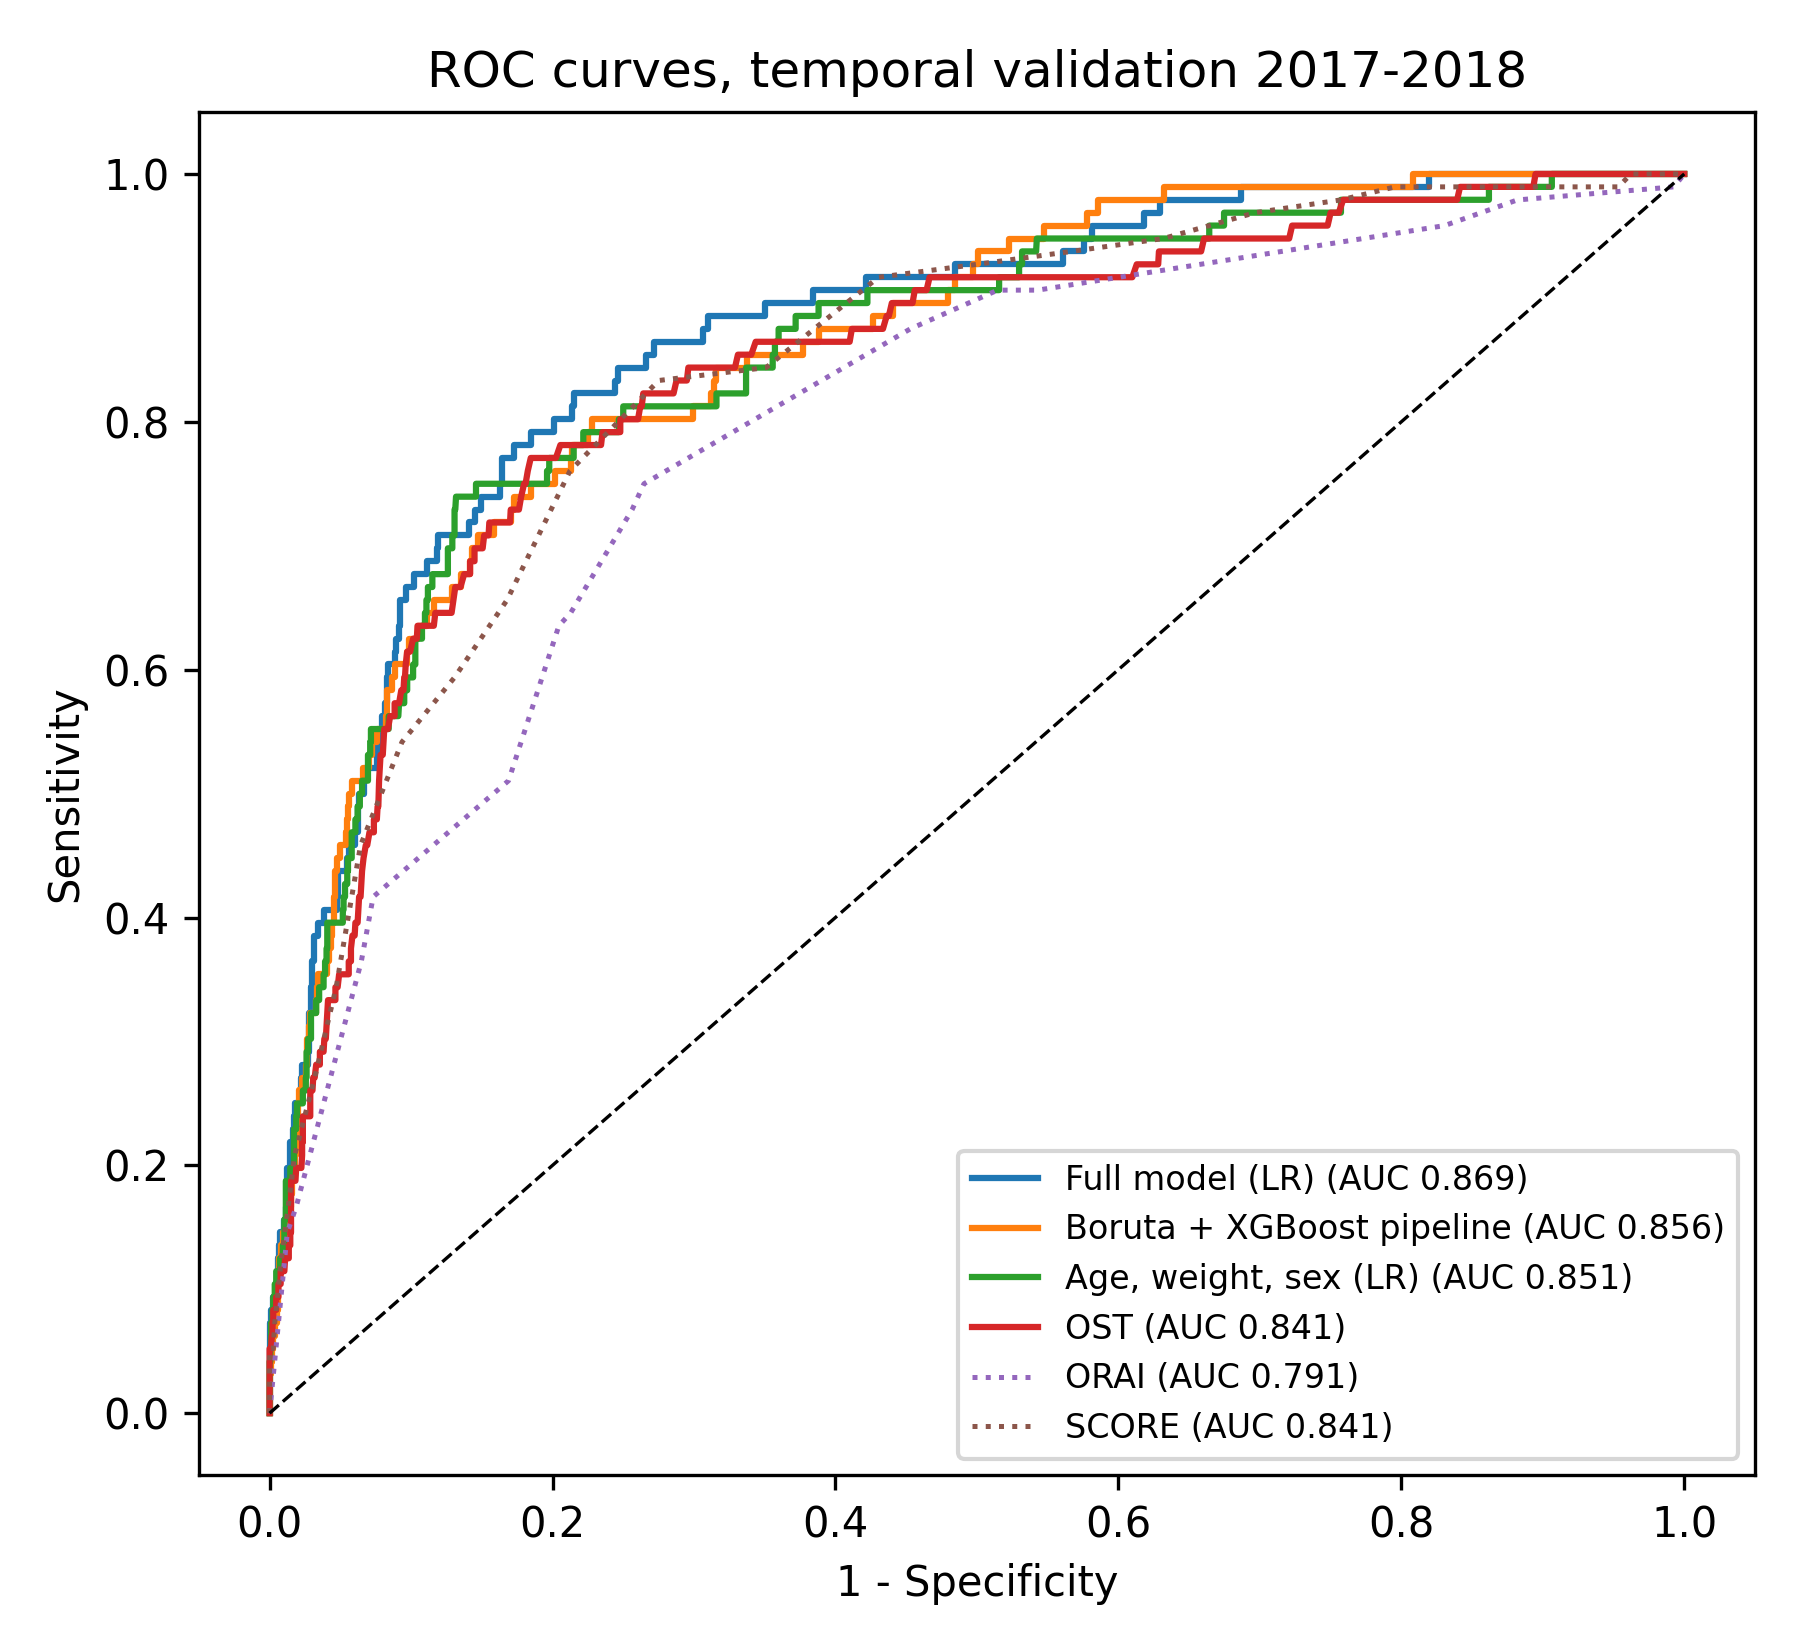
\includegraphics[width=0.6\textwidth]{fig3_roc.png}
\caption{Receiver operating characteristic curves in the temporal validation set (2017--2018) for the full model and the simple or published benchmarks (ORAI and SCORE dotted).}
\label{fig:roc}
\end{figure}

\subsection{Cases detected at fixed DXA capacity}
Across the held-out cycles (45.5 cases per 1,000 screened), the full model detected more cases than every simple tool at each referral rate (Table~\ref{tab:cases}). At 20\% referral it detected 35.3 cases per 1,000, against 34.2 for the clinical model, 33.6 for the sex-specific OST, 33.1 for the three-variable model and 32.5 for OST. Its gain over OST was 2.3--3.0 cases per 1,000 at referral rates of 15\%--30\% (6.9\%--8.6\% more cases), all with CIs excluding zero: one additional case for every 330--430 people screened. The clinical model captured about 60\% of this gain (1.7 of 2.8 per 1,000 at 20\% referral). In the population not routinely screened (216 cases), the gain was 2.3 (0.9--3.9) per 1,000, or 12\% more cases, and in all participants with survey weights it was 2.4 (0.5--4.5) (Supplementary Table~\ref{tab:casesstrata}). At OST's published cut-offs in 2017--2018, the full model at the same referral rate detected 3 ($-$2 to 8) more of the 96 cases than OST $<2$ and 6 ($-$2 to 14) more than OST $<-1$ (Supplementary Table~\ref{tab:ost}).

\begin{table}[!htbp]
\centering
\caption{Cases detected per 1,000 people screened when a fixed proportion, ranked by each tool, is referred for DXA, from the pooled out-of-cycle predictions of the internal--external cross-validation (9,657 participants; 439 cases, 45.5 per 1,000). Referral was applied within each cycle; ties were broken at random (estimates averaged over 200 draws). $\Delta$, full model minus comparator, with 95\% CIs from 1,000 bootstrap resamples within cycles (conditional on the fitted models); \% more, relative increase; per extra case, people screened per additional case found ($1{,}000/\Delta$) with the same number of scans. Clinical + lab: without race/ethnicity, income and education. Clinical: also without laboratory tests (19 predictors).}
\label{tab:cases}
\footnotesize
\setlength{\tabcolsep}{2.5pt}
\resizebox{\textwidth}{!}{%
\begin{tabular}{ccccccccccc}
\toprule
 & \multicolumn{6}{c}{Cases detected per 1,000 screened} & \multicolumn{2}{c}{Full model vs OST} & \multicolumn{2}{c}{Full model vs clinical} \\
\cmidrule(lr){2-7}\cmidrule(lr){8-9}\cmidrule(lr){10-11}
DXA scans per 1,000 & Full & Clinical + lab & Clinical & Age, weight, sex & OST, sex-specific & OST & $\Delta$ (95\% CI); \% more & Per extra case & $\Delta$ (95\% CI) & Per extra case \\
\midrule
150 & 31.8 & 31.5 & 30.2 & 29.2 & 29.4 & 29.5 & 2.3 (0.5--4.0); 7.9\% & 432 & 1.6 (0.0--2.9) & 644 \\
200 & 35.3 & 35.0 & 34.2 & 33.1 & 33.6 & 32.5 & 2.8 (1.0--4.3); 8.6\% & 358 & 1.1 ($-$0.2 to 2.4) & 878 \\
250 & 38.3 & 37.3 & 36.3 & 36.0 & 36.1 & 35.3 & 3.0 (1.4--4.7); 8.5\% & 333 & 2.0 (0.7--3.0) & 508 \\
300 & 40.0 & 39.2 & 38.9 & 37.8 & 38.0 & 37.4 & 2.6 (0.9--3.6); 6.9\% & 386 & 1.0 (0.2--2.1) & 966 \\
\bottomrule
\end{tabular}}
\end{table}

\subsection{Calibration and clinical utility}
The full model was well calibrated internally (cross-fitted slope 0.99) and in 2017--2018 (Brier score 0.038; calibration-in-the-large 0.09, $-$0.16 to 0.29) (Figure~\ref{fig:cal}). Across thresholds of 2\%--15\%, every model had higher net benefit than referring everyone or no one; ORAI had the lowest, and the differences between the others were small relative to their uncertainty (Figure~\ref{fig:dca}; Supplementary Table~\ref{tab:nb}). At a threshold of 10\%, net benefit was 0.022 for the full model and 0.018 for OST, or 2.2 versus 1.8 net true positives per 100 people screened.

\begin{figure}[!htbp]
\centering
\begin{minipage}{0.46\textwidth}\centering
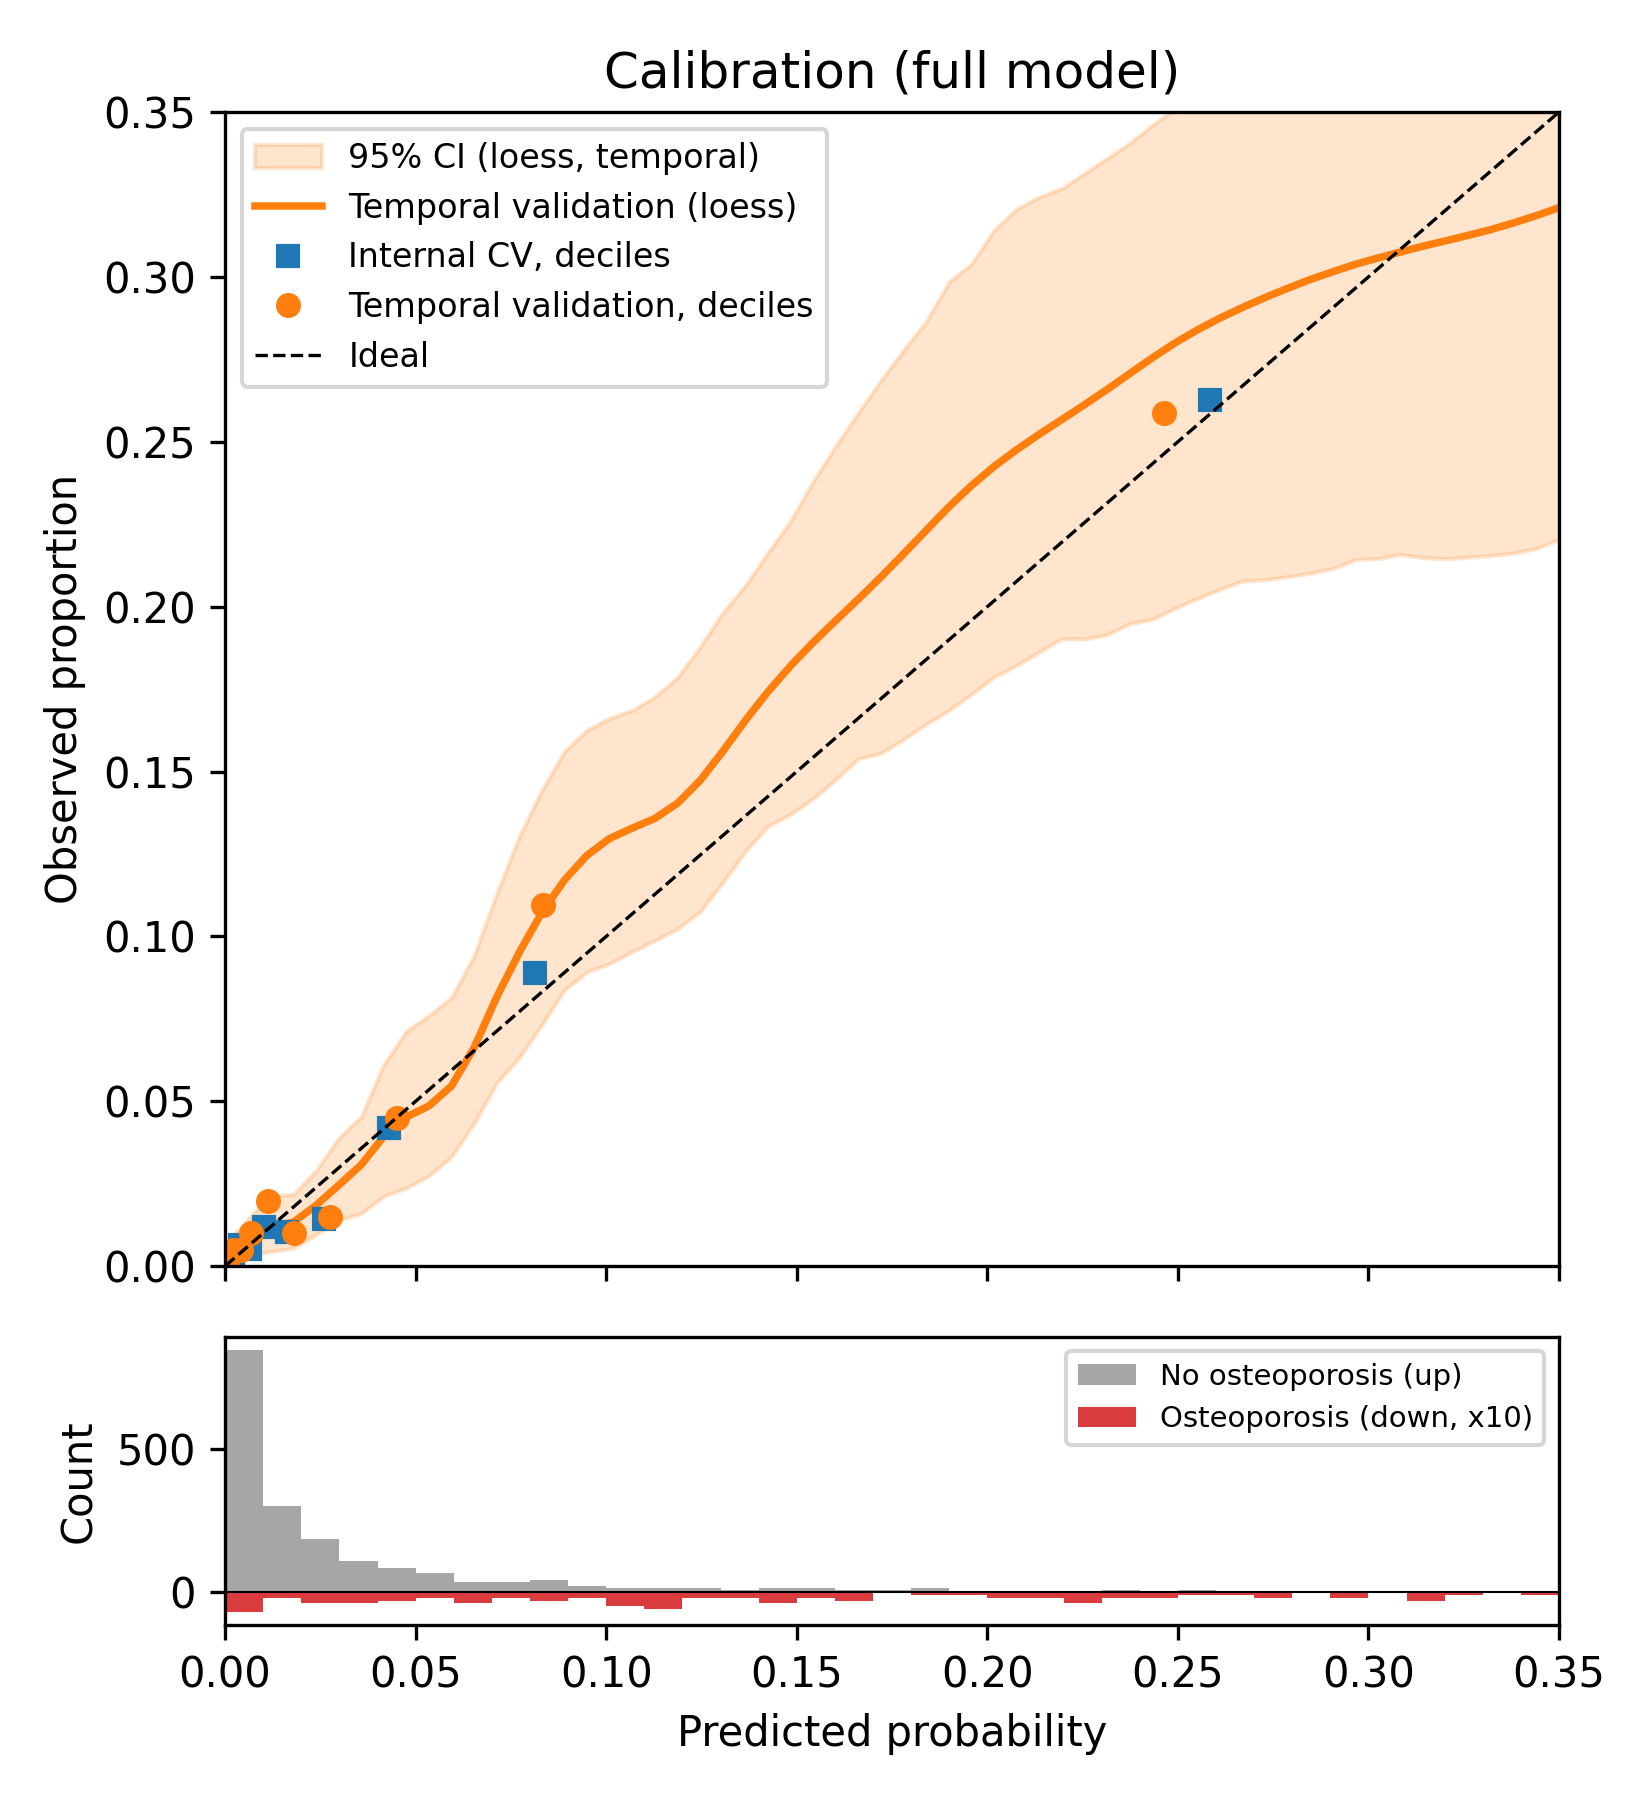
\includegraphics[width=\linewidth]{fig4_calibration.png}
\caption{Calibration of the full model: deciles of predicted risk internally (cross-fitted) and in temporal validation, and a loess curve for the validation set with a 95\% bootstrap band (200 replicates); dashed line, perfect calibration. The axes stop at 0.35 (98th percentile of predictions). Lower panel: predicted risks of participants without (up) and with (down, counts $\times$10) osteoporosis.}
\label{fig:cal}
\end{minipage}\hfill
\begin{minipage}{0.52\textwidth}\centering
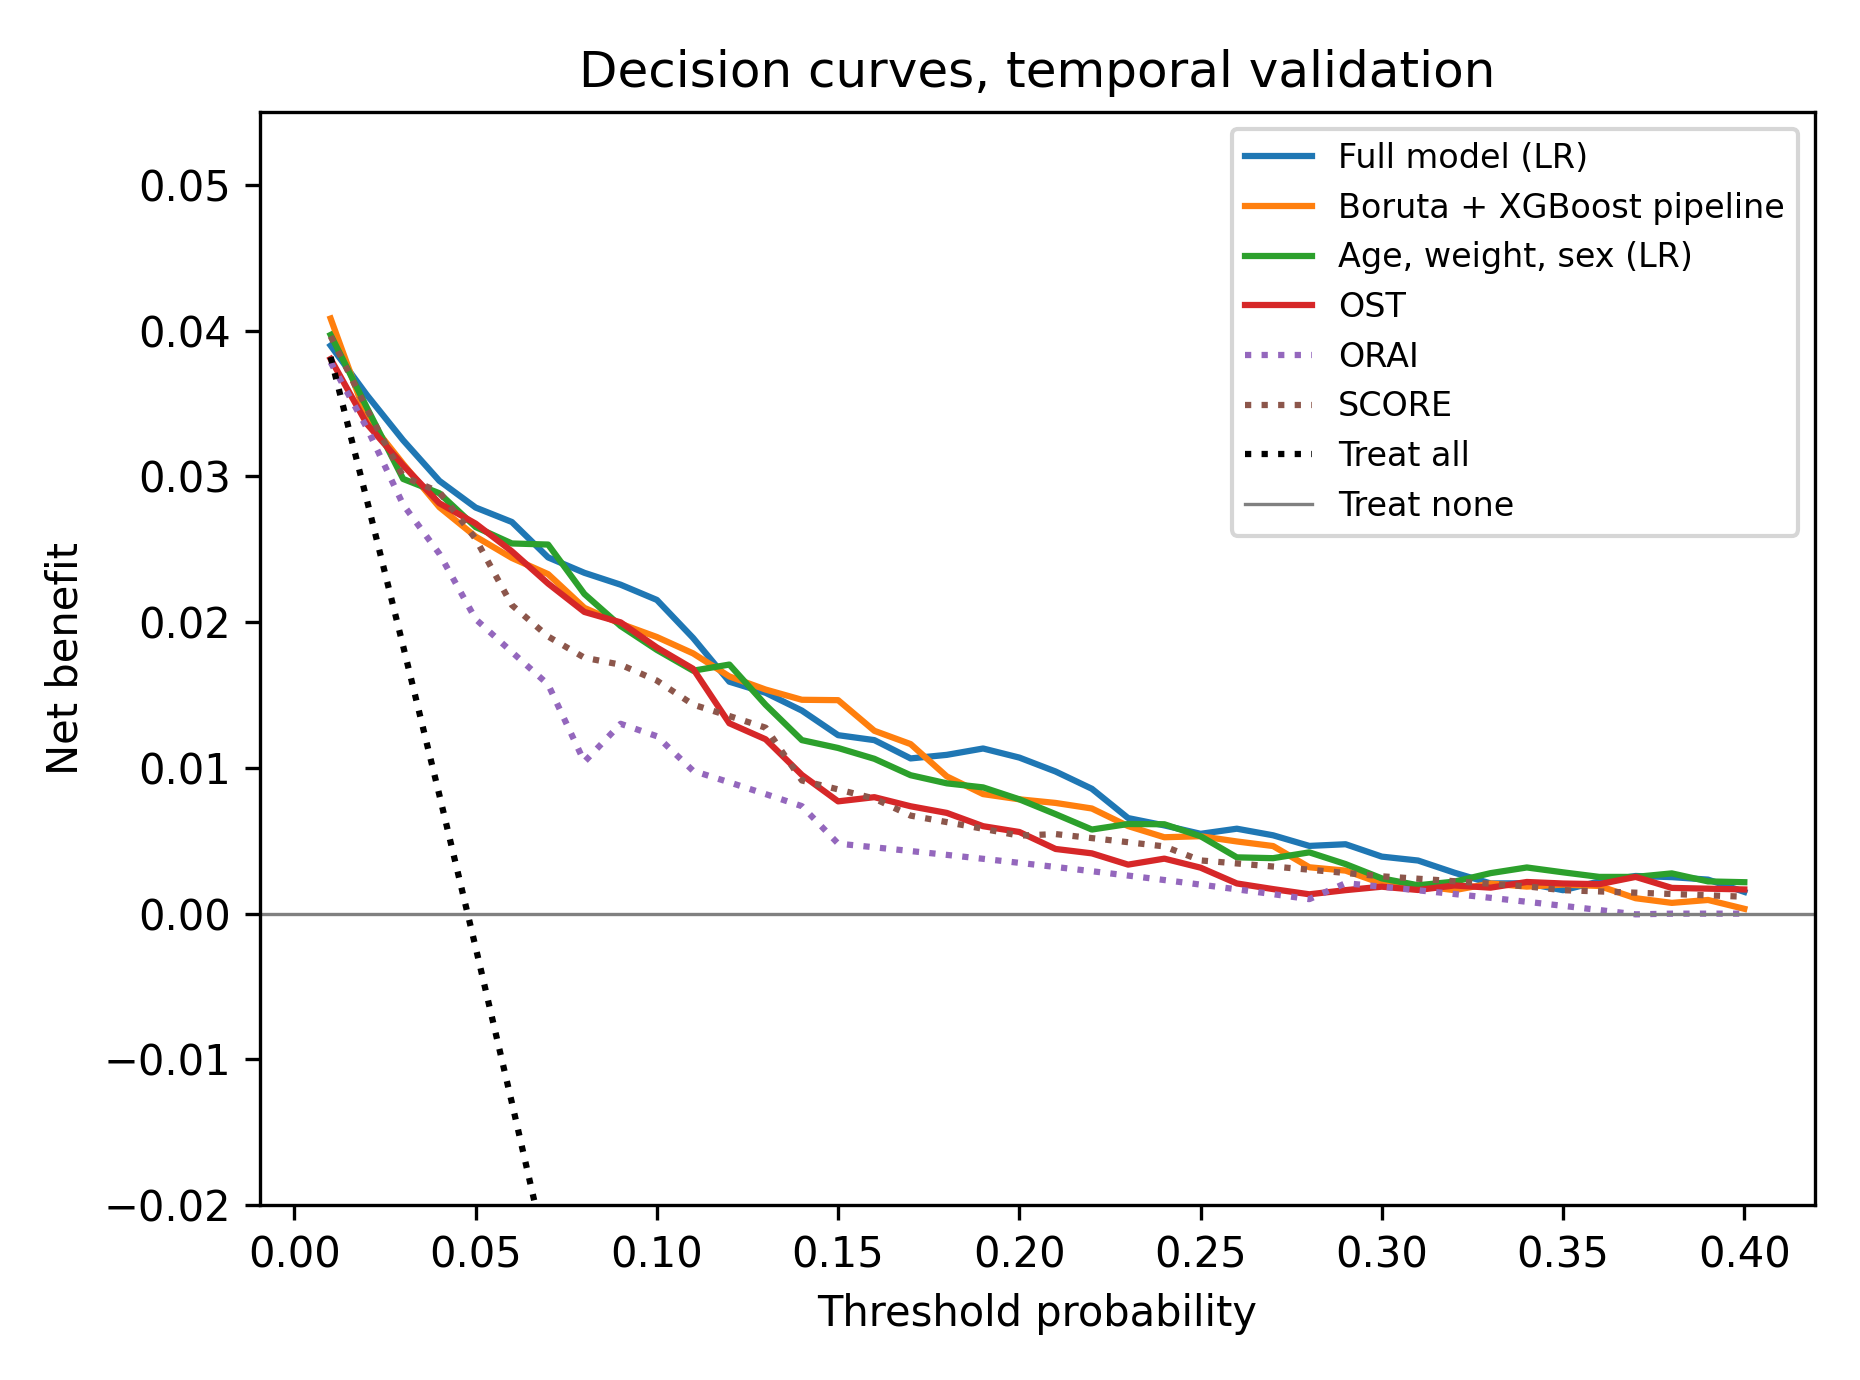
\includegraphics[width=\linewidth]{fig5_decision_curve.png}
\caption{Decision curves in the temporal validation set over threshold probabilities of 2\%--15\% (OST, ORAI and SCORE recalibrated to probabilities).}
\label{fig:dca}
\end{minipage}
\end{figure}

Weighted to the 2017--2018 population, the full model's AUROC was 0.889, against 0.870 for the three-variable model and 0.868 for OST, and 0.872 (0.812--0.934) with non-response adjustment. Non-response factors reached 32.5, but trimming or capping them gave AUROCs of 0.870--0.888 and gains over OST of 0.021--0.025 (Supplementary Table~\ref{tab:wtrim}).

\subsection{Subgroups and clinical strata}
In 2017--2018 the full model discriminated similarly in women and men (AUROC 0.853 and 0.820) but, at the global threshold, detected 61 of 72 cases in women and 16 of 24 in men; sex-specific thresholds raised sensitivity in men to 0.750 with fewer total referrals (Supplementary Table~\ref{tab:fair}). Non-Hispanic Asian adults had a high prevalence (7.3\%) and an AUROC of 0.904; other minority groups had 4--8 cases each.

Across all five cycles (Supplementary Table~\ref{tab:casesstrata}), the full model exceeded OST by 0.031 (0.009--0.054) in women aged 50--64 and 0.029 (0.009--0.048) in women aged 65 or older, and by 0.025 ($-$0.024 to 0.078) and 0.019 ($-$0.015 to 0.056) in men aged 50--69 and $\ge$70; at 20\% referral within each stratum, differences in cases detected had CIs including zero. In 2017--2018, OST $<2$ referred 71.1\% of women aged 65 or older and 59.8\% of men aged 70 or older, against 55.0\% and 30.3\% for the full model at its global threshold (Table~\ref{tab:strata}). All stratum comparisons are exploratory.

\begin{table}[!htbp]
\centering
\caption{Performance in clinical strata of the temporal validation set. AUROC of each model; $\Delta$, full model minus OST (paired bootstrap 95\% CI). The last two columns give cases detected and the proportion referred by the full model at its global Youden threshold (4.8\%) and by OST $<2$ (no fitting). Exploratory; not part of the testing hierarchy.}
\label{tab:strata}
\footnotesize
\setlength{\tabcolsep}{3pt}
\resizebox{\textwidth}{!}{%
\begin{tabular}{lrrcccccccc}
\toprule
 & & & \multicolumn{5}{c}{AUROC} & & \multicolumn{2}{c}{Detected, referred} \\
\cmidrule(lr){4-8}\cmidrule(lr){10-11}
Stratum & $n$ & Cases & Full & Age, weight, sex & OST & SCORE & ORAI & $\Delta$ vs OST (95\% CI) & Full model & OST $<2$ \\
\midrule
Women 50--64 years & 547 & 27 & 0.818 & 0.804 & 0.804 & 0.838 & 0.749 & 0.014 ($-$0.030 to 0.065) & 18/27, 27.4\% & 21/27, 35.5\% \\
Women $\ge$65 years & 311 & 45 & 0.836 & 0.811 & 0.811 & 0.807 & 0.783 & 0.025 ($-$0.019 to 0.068) & 43/45, 55.0\% & 42/45, 71.1\% \\
Men 50--69 years & 787 & 9 & 0.813 & 0.733 & 0.734 & 0.751 & 0.787 & 0.080 (0.013--0.152) & 6/9, 5.8\% & 6/9, 19.4\% \\
Men $\ge$70 years & 363 & 15 & 0.741 & 0.732 & 0.733 & 0.756 & 0.629 & 0.008 ($-$0.074 to 0.100) & 10/15, 30.3\% & 14/15, 59.8\% \\
\bottomrule
\end{tabular}}
\end{table}


\subsection{Sensitivity analyses}
The conclusions did not change in any sensitivity analysis (Supplementary Tables~\ref{tab:sens} and~\ref{tab:scanner}): the full model's AUROC was 0.840--0.885 and exceeded OST wherever OST was evaluated, and across all versions of the analysis the gain of the best model over OST was 0.028--0.045 (Supplementary Table~\ref{tab:versions}).

% ================================================================= 4 Discussion
\section{Discussion}

\subsection{Principal findings}
In 9,657 older US adults neither diagnosed with nor treated for osteoporosis, penalised logistic regression with 35 predictors identified hip osteoporosis with a pooled AUROC of 0.881 across five held-out cycles. It exceeded OST by 0.024 and an age--weight--sex model by 0.019, consistently but by an amount of uncertain clinical relevance: about 3 additional cases per 1,000 people screened at a fixed DXA capacity, about 60\% of which came from clinical items alone. Equally tuned ML did not outperform logistic regression.

\subsection{Comparison with previous studies}
Our results agree with systematic reviews concluding that simple tools based on age and weight perform as well as more complex instruments \cite{rubin2013,nayak2015}. OST's pooled AUROC of 0.856 in both sexes lies at the upper end of the ranges reported in women \cite{geusens2002,rud2007,gourlay2008} and in men \cite{adler2003,lynn2008,diem2017} separately; SCORE performed like OST and ORAI worse, as before \cite{gourlay2008}.

As in KNHANES \cite{shim2020}, ML did not outperform logistic regression. NHANES-based models have reported similar AUROCs (0.81--0.85) \cite{tang2023,zhangy2025,zhang2025}, but with random splits and, mostly, no simple comparator; the larger gain over OST reported for one gradient-boosting model (0.83 vs 0.78) \cite{zhangy2025} may reflect differences in outcome, cohort and tuning. In our re-implementation of one published pipeline \cite{zhang2025}, every combination had an accuracy of 0.954--0.957, close to the 95.5\% obtained by predicting no osteoporosis for everyone, including SVMs with AUROC as low as 0.653 (Supplementary Table~\ref{tab:reimpl}): accuracy cannot rank models for an uncommon condition.

\subsection{How much do additional predictors and machine learning add?}
Most of the discriminative information lay in age, weight and sex; FRAX-type risk factors and medical history added only 0.001 beyond body size and socio-demographic factors (Supplementary Table~\ref{tab:incr}). The relations are largely monotonic and additive, so flexible models have little to exploit: tuned boosting models chose stumps or shallow trees, and splines added nothing. Equal tuning was essential to this conclusion: with default settings, ML families trailed LR by up to 0.035 (Supplementary Table~\ref{tab:tuned}), and comparing a tuned ML model with an untuned regression, or the reverse, could mislead either way \cite{christodoulou2019}.

Our margin of $\pm$0.02 was a judgement, not an external standard. By it, the ML families were equivalent to LR, whereas the full model was better than OST and age, weight and sex but neither equivalent to them nor demonstrably better by a relevant amount \cite{dehond2022}. Whether one additional case per 330--430 people screened justifies a tool that needs 35 inputs, including a biochemistry panel, vitamin D and income, depends on the cost of collecting the inputs, which we did not model. A model of 19 clinical items obtained about two-thirds of the AUROC gain and 60\% of the gain in cases, and laboratory tests and race, income and education each added about 0.005 and up to 1.2 cases per 1,000 (Table~\ref{tab:cases}). Where the clinical items are reliably recorded, part of the gain may be had at little cost, but parental hip fracture, glucocorticoid use and alcohol are often missing or inaccurate in routine records, so such a model needs its own validation. A sex-specific OST, which costs nothing, recovered about a quarter of the AUROC gain but few cases ($-$0.1 to 1.0 per 1,000).

\subsection{Why not FRAX?}
FRAX estimates the 10-year probability of fracture \cite{kanis2008} and guides treatment, but our question is who should have DXA. For that purpose, FRAX without BMD discriminated low BMD less well than OST or SCORE in women aged 50--64 years (AUROC 0.60 vs 0.72--0.73) \cite{crandall2014} and in older men (0.62 vs 0.68) \cite{diem2017}, and NHANES lacks several FRAX inputs (for example, current glucocorticoid use and secondary osteoporosis), so we used tools designed to predict low BMD.

\subsection{Calibration, thresholds and implementation}
Class weighting and SMOTE inflated predicted risks until recalibration \cite{vandengoorbergh2022}, so models used for absolute risk should be fitted on the original class distribution. The threshold mattered more than the model: one set for 90\% sensitivity detected 86 of 96 cases while referring 39\% of participants (Supplementary Table~\ref{tab:ops}). The operating point should be set locally from DXA capacity, and, because calibration varied between cycles (observed-to-expected ratio 0.84--1.16), the intercept should be recalibrated locally before predicted risks are used.

OST, a sex-specific OST and the three-variable model can be computed automatically from routinely recorded age, sex and weight; the full model also needs blood tests and income. All the regression models reduce to a single linear equation (Supplementary Table~\ref{tab:coef}), whereas boosting models would need software integration for no gain. A model card summarises intended use, inputs, performance and monitoring (Supplementary Table~\ref{tab:modelcard}).

\subsection{Subgroups and fairness}
A single threshold detected only two-thirds of cases in men, reflecting their low baseline risk; sex-specific thresholds improved this without more referrals, but raising detection in men further is a policy decision \cite{uspstf2025}. In women aged 65 or older, who are screened regardless of risk, a tool matters mainly for ordering patients when capacity is limited. Where a tool would decide who is scanned at all, in younger postmenopausal women and in men, the AUROC gains were similar but the differences in cases detected were small and uncertain, so these data cannot choose between tools there. Removing race/ethnicity changed discrimination little, and with 4--8 cases in most minority groups our data cannot show whether any tool performs less well in a particular group \cite{paulus2020,vyas2020}.

\subsection{Strengths and limitations}
Strengths include a large national probability sample with standardised DXA, restricted to the intended screening population; IECV across all five cycles, with the tuning of every model family nested inside each development set and equivalence tests applied in both directions, complemented by a temporal split and a bootstrap including model refitting; head-to-head comparison with three established screening indices and a sex-specific OST; assessment of calibration, net benefit and cases detected at fixed capacity; and full reproducibility from public data and open code, with every analysis version reported.

The study also has limitations. First, it is cross-sectional: the models detect existing osteoporosis, not future fractures. Second, the outcome, cohort, estimand, margin and benchmarks were revised after earlier versions had examined the data (Supplementary Table~\ref{tab:versions}); the predictor list, outcome and choice of LR were fixed on data that overlap the IECV folds; and no untouched data exist, because the 2021--2023 NHANES cycle has released no femur DXA data, so the frozen model and code are public for future validation. Third, the hip-only outcome underestimates osteoporosis defined at any site \cite{sarafrazi2021}, although spine-inclusive outcomes gave similar conclusions. Fourth, scanners, laboratory methods and the alcohol questionnaire changed between cycles; shifted T-scores, omission of laboratory predictors or alcohol, and same-scanner development gave similar results. Fifth, risk factors were self-reported, glucocorticoid use was ever rather than current, and ORAI and SCORE had to be adapted, which may understate them. Sixth, models were unweighted and participants without DXA differed from the cohort, so the results may not fully represent the US population aged 50 or older. Seventh, imputation was single; the IECV CIs are approximate because development sets overlap, and the case-count CIs are conditional on the fitted models; and men, younger women and minority groups had few cases. Finally, all data are from the United States; external validation is needed, particularly where DXA access is most limited.

\section{Conclusion}
In older US adults neither diagnosed with nor treated for osteoporosis, equally tuned machine learning did not outperform logistic regression, and 35 predictors added about 0.02 in AUROC to OST and to age, weight and sex, or about 3 more cases per 1,000 people screened at the same DXA capacity, two-thirds of it obtainable from clinical items alone. Simple tools capture most of the achievable discrimination; whether the remainder is worth a complex tool is a decision for each health system, and the choice of threshold, including whether it is applied to men, matters more than the algorithm.


\begin{thebibliography}{99}\small

\bibitem{compston2019} Compston JE, McClung MR, Leslie WD. Osteoporosis. Lancet. 2019;393(10169):364--376. \href{https://doi.org/10.1016/S0140-6736(18)32112-3}{doi:10.1016/S0140-6736(18)32112-3}

\bibitem{sarafrazi2021} Sarafrazi N, Wambogo EA, Shepherd JA. Osteoporosis or low bone mass in older adults: United States, 2017--2018. NCHS Data Brief No.\ 405. Hyattsville, MD: National Center for Health Statistics; 2021. \href{https://dx.doi.org/10.15620/cdc:103477}{doi:10.15620/cdc:103477}

\bibitem{kanis1994} Kanis JA, Melton LJ 3rd, Christiansen C, Johnston CC, Khaltaev N. The diagnosis of osteoporosis. J Bone Miner Res. 1994;9(8):1137--1141. \href{https://doi.org/10.1002/jbmr.5650090802}{doi:10.1002/jbmr.5650090802}

\bibitem{uspstf2025} US Preventive Services Task Force; Nicholson WK, Silverstein M, Wong JB, et al. Screening for osteoporosis to prevent fractures: US Preventive Services Task Force recommendation statement. JAMA. 2025;333(6):498. \href{https://doi.org/10.1001/jama.2024.27154}{doi:10.1001/jama.2024.27154}

\bibitem{geusens2002} Geusens P, Hochberg MC, van der Voort DJ, Pols H, van der Klift M, Siris E, et al. Performance of risk indices for identifying low bone density in postmenopausal women. Mayo Clin Proc. 2002;77(7):629--637. \href{https://doi.org/10.4065/77.7.629}{doi:10.4065/77.7.629}

\bibitem{koh2001} Koh LK, Sedrine WB, Torralba TP, et al. A simple tool to identify Asian women at increased risk of osteoporosis. Osteoporos Int. 2001;12(8):699--705. \href{https://doi.org/10.1007/s001980170070}{doi:10.1007/s001980170070}

\bibitem{cadarette2000} Cadarette SM, Jaglal SB, Kreiger N, McIsaac WJ, Darlington GA, Tu JV. Development and validation of the Osteoporosis Risk Assessment Instrument to facilitate selection of women for bone densitometry. CMAJ. 2000;162(9):1289--1294.

\bibitem{lydick1998} Lydick E, Cook K, Turpin J, Melton M, Stine R, Byrnes C. Development and validation of a simple questionnaire to facilitate identification of women likely to have low bone density. Am J Manag Care. 1998;4(1):37--48.

\bibitem{rud2007} Rud B, Hilden J, Hyldstrup L, Hr\'{o}bjartsson A. Performance of the Osteoporosis Self-Assessment Tool in ruling out low bone mineral density in postmenopausal women: a systematic review. Osteoporos Int. 2007;18(9):1177--1187. \href{https://doi.org/10.1007/s00198-006-0319-3}{doi:10.1007/s00198-006-0319-3}

\bibitem{gourlay2008} Gourlay ML, Powers JM, Lui LY, Ensrud KE. Clinical performance of osteoporosis risk assessment tools in women aged 67 years and older. Osteoporos Int. 2008;19(8):1175--1183. \href{https://doi.org/10.1007/s00198-007-0555-1}{doi:10.1007/s00198-007-0555-1}

\bibitem{rubin2013} Rubin KH, Friis-Holmberg T, Hermann AP, Abrahamsen B, Brixen K. Risk assessment tools to identify women with increased risk of osteoporotic fracture: complexity or simplicity? A systematic review. J Bone Miner Res. 2013;28(8):1701--1717. \href{https://doi.org/10.1002/jbmr.1956}{doi:10.1002/jbmr.1956}

\bibitem{nayak2015} Nayak S, Edwards DL, Saleh AA, Greenspan SL. Systematic review and meta-analysis of the performance of clinical risk assessment instruments for screening for osteoporosis or low bone density. Osteoporos Int. 2015;26(5):1543--1554. \href{https://doi.org/10.1007/s00198-015-3025-1}{doi:10.1007/s00198-015-3025-1}

\bibitem{adler2003} Adler RA, Tran MT, Petkov VI. Performance of the Osteoporosis Self-assessment Screening Tool for osteoporosis in American men. Mayo Clin Proc. 2003;78(6):723--727. \href{https://doi.org/10.4065/78.6.723}{doi:10.4065/78.6.723}

\bibitem{lynn2008} Lynn HS, Woo J, Leung PC, Barrett-Connor EL, Nevitt MC, Cauley JA, et al. An evaluation of osteoporosis screening tools for the osteoporotic fractures in men (MrOS) study. Osteoporos Int. 2008;19(7):1087--1092. \href{https://doi.org/10.1007/s00198-007-0553-3}{doi:10.1007/s00198-007-0553-3}

\bibitem{diem2017} Diem SJ, Peters KW, Gourlay ML, Schousboe JT, Taylor BC, Orwoll ES, et al. Screening for osteoporosis in older men: operating characteristics of proposed strategies for selecting men for BMD testing. J Gen Intern Med. 2017;32(11):1235--1241. \href{https://doi.org/10.1007/s11606-017-4153-4}{doi:10.1007/s11606-017-4153-4}

\bibitem{cass2006} Cass AR, Shepherd AJ, Carlson CA. Osteoporosis risk assessment and ethnicity: validation and comparison of 2 clinical risk stratification instruments. J Gen Intern Med. 2006;21(6):630--635. \href{https://doi.org/10.1111/j.1525-1497.2006.00459.x}{doi:10.1111/j.1525-1497.2006.00459.x}

\bibitem{crandall2014} Crandall CJ, Larson J, Gourlay ML, Donaldson MG, LaCroix A, Cauley JA, et al. Osteoporosis screening in postmenopausal women 50 to 64 years old: comparison of US Preventive Services Task Force strategy and two traditional strategies in the Women's Health Initiative. J Bone Miner Res. 2014;29(7):1661--1666. \href{https://doi.org/10.1002/jbmr.2174}{doi:10.1002/jbmr.2174}

\bibitem{shim2020} Shim JG, Kim DW, Ryu KH, Cho EA, Ahn JH, Kim JI, et al. Application of machine learning approaches for osteoporosis risk prediction in postmenopausal women. Arch Osteoporos. 2020;15(1):169. \href{https://doi.org/10.1007/s11657-020-00802-8}{doi:10.1007/s11657-020-00802-8}

\bibitem{suh2023} Suh B, Yu H, Kim H, Lee S, Kong S, Kim JW, et al. Interpretable deep-learning approaches for osteoporosis risk screening and individualized feature analysis using large population-based data: model development and performance evaluation. J Med Internet Res. 2023;25:e40179. \href{https://doi.org/10.2196/40179}{doi:10.2196/40179}

\bibitem{tang2023} Tang Y, Liu J, Tian C, Feng Z, Zhang X, Xia Y, et al. A novel primary osteoporosis screening tool (POST) for adults aged 50 years and over. Endocrine. 2023;82(1):190--200. \href{https://doi.org/10.1007/s12020-023-03442-3}{doi:10.1007/s12020-023-03442-3}

\bibitem{zhangy2025} Zhang Y, Ma M, Tian C, Liu J, Duan Z, Huang X, et al. A machine-learning-based osteoporosis screening tool integrating the Shapley Additive exPlanation (SHAP) method: model development and validation study. Arch Osteoporos. 2025;20(1):134. \href{https://doi.org/10.1007/s11657-025-01602-8}{doi:10.1007/s11657-025-01602-8}

\bibitem{zhang2025} Zhang D, Yang X, Wang F, Qiu C, Chai Y, Fang D. Comparative analysis of feature extraction methods and machine learning models for predicting osteoporosis prevalence. J Med Syst. 2025;49(1):72. \href{https://doi.org/10.1007/s10916-025-02203-1}{doi:10.1007/s10916-025-02203-1}

\bibitem{christodoulou2019} Christodoulou E, Ma J, Collins GS, Steyerberg EW, Verbakel JY, Van Calster B. A systematic review shows no performance benefit of machine learning over logistic regression for clinical prediction models. J Clin Epidemiol. 2019;110:12--22. \href{https://doi.org/10.1016/j.jclinepi.2019.02.004}{doi:10.1016/j.jclinepi.2019.02.004}

\bibitem{vandengoorbergh2022} van den Goorbergh R, van Smeden M, Timmerman D, Van Calster B. The harm of class imbalance corrections for risk prediction models: illustration and simulation using logistic regression. J Am Med Inform Assoc. 2022;29(9):1525--1534. \href{https://doi.org/10.1093/jamia/ocac093}{doi:10.1093/jamia/ocac093}

\bibitem{collins2024} Collins GS, Moons KGM, Dhiman P, et al. TRIPOD+AI statement: updated guidance for reporting clinical prediction models that use regression or machine learning methods. BMJ. 2024;385:e078378. \href{https://doi.org/10.1136/bmj-2023-078378}{doi:10.1136/bmj-2023-078378}

\bibitem{johnson2013} Johnson CL, Paulose-Ram R, Ogden CL, et al. National Health and Nutrition Examination Survey: analytic guidelines, 1999--2010. Vital Health Stat 2. 2013;(161):1--24.

\bibitem{johnson2014} Johnson CL, Dohrmann SM, Burt VL, Mohadjer LK. National Health and Nutrition Examination Survey: sample design, 2011--2014. Vital Health Stat 2. 2014;(162):1--33.

\bibitem{looker1998} Looker AC, Wahner HW, Dunn WL, et al. Updated data on proximal femur bone mineral levels of US adults. Osteoporos Int. 1998;8(5):468--490. \href{https://doi.org/10.1007/s001980050093}{doi:10.1007/s001980050093}

\bibitem{watts2013} Watts NB, Leslie WD, Foldes AJ, Miller PD. 2013 International Society for Clinical Densitometry Position Development Conference: Task Force on Normative Databases. J Clin Densitom. 2013;16(4):472--481. \href{https://doi.org/10.1016/j.jocd.2013.08.001}{doi:10.1016/j.jocd.2013.08.001}

\bibitem{baim2008} Baim S, Binkley N, Bilezikian JP, Kendler DL, Hans DB, et al. Official Positions of the International Society for Clinical Densitometry and executive summary of the 2007 ISCD Position Development Conference. J Clin Densitom. 2008;11(1):75--91. \href{https://doi.org/10.1016/j.jocd.2007.12.007}{doi:10.1016/j.jocd.2007.12.007}

\bibitem{wright2014} Wright NC, Looker AC, Saag KG, Curtis JR, Delzell ES, Randall S, Dawson-Hughes B. The recent prevalence of osteoporosis and low bone mass in the United States based on bone mineral density at the femoral neck or lumbar spine. J Bone Miner Res. 2014;29(11):2520--2526. \href{https://doi.org/10.1002/jbmr.2269}{doi:10.1002/jbmr.2269}

\bibitem{vanbuuren2011} van Buuren S, Groothuis-Oudshoorn K. mice: Multivariate imputation by chained equations in R. J Stat Softw. 2011;45(3):1--67. \href{https://doi.org/10.18637/jss.v045.i03}{doi:10.18637/jss.v045.i03}

\bibitem{perperoglou2019} Perperoglou A, Sauerbrei W, Abrahamowicz M, Schmid M. A review of spline function procedures in R. BMC Med Res Methodol. 2019;19(1):46. \href{https://doi.org/10.1186/s12874-019-0666-3}{doi:10.1186/s12874-019-0666-3}

\bibitem{chen2016} Chen T, Guestrin C. XGBoost: a scalable tree boosting system. In: Proceedings of the 22nd ACM SIGKDD International Conference on Knowledge Discovery and Data Mining; 2016:785--794. \href{https://doi.org/10.1145/2939672.2939785}{doi:10.1145/2939672.2939785}

\bibitem{ke2017} Ke G, Meng Q, Finley T, et al. LightGBM: a highly efficient gradient boosting decision tree. In: Advances in Neural Information Processing Systems 30 (NIPS 2017). \url{https://proceedings.neurips.cc/paper_files/paper/2017/hash/6449f44a102fde848669bdd9eb6b76fa-Abstract.html}

\bibitem{prokhorenkova2018} Prokhorenkova L, Gusev G, Vorobev A, Dorogush AV, Gulin A. CatBoost: unbiased boosting with categorical features. In: Advances in Neural Information Processing Systems 31 (NeurIPS 2018). \url{https://proceedings.neurips.cc/paper_files/paper/2018/hash/14491b756b3a51daac41c24863285549-Abstract.html}

\bibitem{chawla2002} Chawla NV, Bowyer KW, Hall LO, Kegelmeyer WP. SMOTE: synthetic minority over-sampling technique. J Artif Intell Res. 2002;16:321--357. \href{https://doi.org/10.1613/jair.953}{doi:10.1613/jair.953}

\bibitem{akiba2019} Akiba T, Sano S, Yanase T, Ohta T, Koyama M. Optuna: a next-generation hyperparameter optimization framework. In: Proceedings of the 25th ACM SIGKDD International Conference on Knowledge Discovery \& Data Mining; 2019:2623--2631. \href{https://doi.org/10.1145/3292500.3330701}{doi:10.1145/3292500.3330701}

\bibitem{kursa2010} Kursa MB, Rudnicki WR. Feature selection with the Boruta package. J Stat Softw. 2010;36(11):1--13. \href{https://doi.org/10.18637/jss.v036.i11}{doi:10.18637/jss.v036.i11}

\bibitem{vyas2020} Vyas DA, Eisenstein LG, Jones DS. Hidden in plain sight -- reconsidering the use of race correction in clinical algorithms. N Engl J Med. 2020;383(9):874--882. \href{https://doi.org/10.1056/NEJMms2004740}{doi:10.1056/NEJMms2004740}

\bibitem{platt2000} Platt JC. Probabilities for SV machines. In: Smola AJ, Bartlett P, Sch\"olkopf B, Schuurmans D, editors. Advances in Large-Margin Classifiers. Cambridge, MA: MIT Press; 2000:61--74. \href{https://doi.org/10.7551/mitpress/1113.003.0008}{doi:10.7551/mitpress/1113.003.0008}

\bibitem{vancalster2019} Van Calster B, McLernon DJ, van Smeden M, Wynants L, Steyerberg EW. Calibration: the Achilles heel of predictive analytics. BMC Med. 2019;17(1):230. \href{https://doi.org/10.1186/s12916-019-1466-7}{doi:10.1186/s12916-019-1466-7}

\bibitem{vickers2006} Vickers AJ, Elkin EB. Decision curve analysis: a novel method for evaluating prediction models. Med Decis Making. 2006;26(6):565--574. \href{https://doi.org/10.1177/0272989X06295361}{doi:10.1177/0272989X06295361}

\bibitem{youden1950} Youden WJ. Index for rating diagnostic tests. Cancer. 1950;3(1):32--35.

\bibitem{dehond2022} de Hond AAH, Steyerberg EW, van Calster B. Interpreting area under the receiver operating characteristic curve. Lancet Digit Health. 2022;4(12):e853--e855. \href{https://doi.org/10.1016/S2589-7500(22)00188-1}{doi:10.1016/S2589-7500(22)00188-1}

\bibitem{holm1979} Holm S. A simple sequentially rejective multiple test procedure. Scand J Stat. 1979;6(2):65--70.

\bibitem{steyerberg2016} Steyerberg EW, Harrell FE Jr. Prediction models need appropriate internal, internal-external, and external validation. J Clin Epidemiol. 2016;69:245--247. \href{https://doi.org/10.1016/j.jclinepi.2015.04.005}{doi:10.1016/j.jclinepi.2015.04.005}

\bibitem{dersimonian1986} DerSimonian R, Laird N. Meta-analysis in clinical trials. Control Clin Trials. 1986;7(3):177--188. \href{https://doi.org/10.1016/0197-2456(86)90046-2}{doi:10.1016/0197-2456(86)90046-2}

\bibitem{inthout2014} IntHout J, Ioannidis JPA, Borm GF. The Hartung-Knapp-Sidik-Jonkman method for random effects meta-analysis is straightforward and considerably outperforms the standard DerSimonian-Laird method. BMC Med Res Methodol. 2014;14:25. \href{https://doi.org/10.1186/1471-2288-14-25}{doi:10.1186/1471-2288-14-25}

\bibitem{hanley1982} Hanley JA, McNeil BJ. The meaning and use of the area under a receiver operating characteristic (ROC) curve. Radiology. 1982;143(1):29--36. \href{https://doi.org/10.1148/radiology.143.1.7063747}{doi:10.1148/radiology.143.1.7063747}

\bibitem{chen2020} Chen TC, Clark J, Riddles MK, Mohadjer LK, Fakhouri THI. National Health and Nutrition Examination Survey, 2015--2018: sample design and estimation procedures. Vital Health Stat 2. 2020;(184):1--35.

\bibitem{raowu1988} Rao JNK, Wu CFJ. Resampling inference with complex survey data. J Am Stat Assoc. 1988;83(401):231--241. \href{https://doi.org/10.1080/01621459.1988.10478591}{doi:10.1080/01621459.1988.10478591}

\bibitem{potter1990} Potter FJ. A study of procedures to identify and trim extreme sampling weights. In: Proceedings of the Survey Research Methods Section, American Statistical Association; 1990:225--230.

\bibitem{lee2011} Lee BK, Lessler J, Stuart EA. Weight trimming and propensity score weighting. PLoS One. 2011;6(3):e18174. \href{https://doi.org/10.1371/journal.pone.0018174}{doi:10.1371/journal.pone.0018174}

\bibitem{lundberg2017} Lundberg SM, Lee SI. A unified approach to interpreting model predictions. In: Advances in Neural Information Processing Systems 30 (NIPS 2017). \url{https://proceedings.neurips.cc/paper/2017/hash/8a20a8621978632d76c43dfd28b67767-Abstract.html}

\bibitem{pedregosa2011} Pedregosa F, Varoquaux G, Gramfort A, et al. Scikit-learn: machine learning in Python. J Mach Learn Res. 2011;12(85):2825--2830. \url{https://jmlr.org/papers/v12/pedregosa11a.html}

\bibitem{kanis2008} Kanis JA, Johnell O, Oden A, Johansson H, McCloskey E. FRAX and the assessment of fracture probability in men and women from the UK. Osteoporos Int. 2008;19(4):385--397. \href{https://doi.org/10.1007/s00198-007-0543-5}{doi:10.1007/s00198-007-0543-5}

\bibitem{paulus2020} Paulus JK, Kent DM. Predictably unequal: understanding and addressing concerns that algorithmic clinical prediction may increase health disparities. NPJ Digit Med. 2020;3:99. \href{https://doi.org/10.1038/s41746-020-0304-9}{doi:10.1038/s41746-020-0304-9}

\bibitem{tibshirani1996} Tibshirani R. Regression shrinkage and selection via the lasso. J R Stat Soc Series B Stat Methodol. 1996;58(1):267--288. \href{https://doi.org/10.1111/j.2517-6161.1996.tb02080.x}{doi:10.1111/j.2517-6161.1996.tb02080.x}

\bibitem{batista2004} Batista GEAPA, Prati RC, Monard MC. A study of the behavior of several methods for balancing machine learning training data. ACM SIGKDD Explor Newsl. 2004;6(1):20--29. \href{https://doi.org/10.1145/1007730.1007735}{doi:10.1145/1007730.1007735}

\end{thebibliography}

\clearpage
\appendix
\section*{Supplementary material}
\renewcommand{\thefigure}{S\arabic{figure}}
\renewcommand{\thetable}{S\arabic{table}}
\setcounter{figure}{0}
\setcounter{table}{0}



\subsection*{Supplementary Methods}

\paragraph{Exclusions.} Osteoporosis medications were bisphosphonates (alendronate, risedronate, ibandronate, zoledronic acid, etidronate), denosumab, raloxifene, bazedoxifene, teriparatide, abaloparatide, romosozumab and calcitonin; 486 excluded participants used one. Participants with a missing answer to the diagnosis question were treated as not diagnosed.

\paragraph{Outcome.} T-scores were (BMD $-$ reference mean)/reference SD, with reference means of 0.858\,g/cm$^2$ (SD 0.120) at the femoral neck and 0.942\,g/cm$^2$ (SD 0.122) at the total hip \cite{looker1998}. Mean femoral neck BMD in women was 0.744--0.753\,g/cm$^2$ in 2005--2010 and 0.729--0.731\,g/cm$^2$ in 2013--2018. The spine-inclusive outcomes were (i) hip or complete-scan L1--L4 T-score $\le -2.5$ and (ii) hip or spine T-score $\le -2.5$ with spine BMD from at least two valid vertebrae (total bone mineral content divided by total projected area) \cite{baim2008}, using the Hologic young white-female spine reference (mean 1.047\,g/cm$^2$, SD 0.110) \cite{sarafrazi2021,wright2014}.

\paragraph{Harmonisation.} Age is top-coded at 85 years in 2005--2006 and at 80 years thereafter, so it was capped at 80 in all cycles. Creatinine from 2005--2006 was recalibrated to the standardised method ($-0.016 + 0.978\times$ measured value). Vitamin D was the LC-MS/MS or LC-MS/MS-equivalent value released for each cycle. Average daily alcohol intake was drinks per drinking day multiplied by drinking days per year, divided by 365; drinking frequency was recorded as a count up to 2013--2014 and as a category in 2017--2018, which we converted to approximate days per year. Values stored as numerical underflow ($<10^{-30}$) were restored to 0. Other laboratory measurements were used as released; their means differed between periods (for example, alkaline phosphatase 72.6 vs 82.6\,U/L; Supplementary Table~\ref{tab:devval}), so we also refitted the model without laboratory predictors. Postmenopausal status was defined as no regular menstrual periods in the past 12 months (which also captures hysterectomy). Responses of ``refused'' or ``don't know'' were set to missing, and borderline diabetes was coded as no diabetes. The analysis stopped automatically if any predictor was entirely missing within a cycle. All predictors were standardised after imputation.

\paragraph{Benchmark scores.} ORAI \cite{cadarette2000}: 15, 9 or 5 points for age $\ge$75, 65--74 or 55--64 years; 9 or 3 points for weight $<$60 or 60--69\,kg; and 2 points for no estrogen use (NHANES records ever rather than current use of female hormones). SCORE \cite{lydick1998}: 5 points if not Black, 4 for rheumatoid arthritis (from the arthritis-type question), 4 for each fracture site (maximum 12; NHANES records hip, wrist and spine fractures of any cause, rather than non-traumatic wrist, rib and hip fractures after age 45), 3 times the first digit of age and 1 for no estrogen use, minus weight in pounds divided by 10 (truncated). Rheumatoid arthritis was used only for SCORE. For the Boruta + XGBoost pipeline, Boruta \cite{kursa2010} selected features from our candidate set on the development data, and XGBoost, tuned with the same budget as the other families, was fitted to them; because the original feature set and outcome differ, this tests the approach rather than the published model.

\paragraph{Re-implementation of the published analysis.} To mirror Zhang et al.\ \cite{zhang2025}, we evaluated all combinations of three feature-selection methods (Boruta, Lasso \cite{tibshirani1996} and XGBoost importance) with four classifiers (LR, SVM, RF and XGBoost) by 10-fold cross-validation on the development set. Features were selected once on the full development set, so these estimates are optimistic.

\paragraph{Model details.} LR-spline used four knots at quantiles with linear extrapolation beyond the boundary knots. The stacking ensemble used RF, XGBoost, LightGBM and CatBoost as base learners with an LR meta-learner. SMOTE-Tomek \cite{batista2004}, used in an earlier version, removed no Tomek links and was identical to SMOTE. Tuned hyperparameters were kept only if they improved on the defaults. Internal calibration was assessed with cross-fitted recalibration. Tuning and selection on the same folds make the internal estimates slightly optimistic but do not affect the temporal estimates.

\paragraph{Incremental value of predictor groups.} Nested LR models added predictor groups in clinical order (age, weight and sex; other body measures and socio-demographic factors; clinical risk factors and history; laboratory tests; race/ethnicity), each developed and validated as the full model.

\paragraph{Predictor importance.} Importance was ranked by mean absolute SHAP value \cite{lundberg2017} in 500 randomly selected development-set participants (permutation explainer, 100 background samples, probability scale before recalibration).

\subsection*{Supplementary Results}

\paragraph{Re-implementation: results.} In 10-fold cross-validation, LR had the highest AUROC with every feature set (0.871--0.879), followed by RF and XGBoost (0.845--0.855, with no consistent order); SVM with default settings performed worst (0.653--0.777). Accuracy was 0.954--0.957 for all 12 combinations, almost identical to the 95.5\% of the development set without osteoporosis (Supplementary Table~\ref{tab:reimpl}; selected predictors in the code repository).

\paragraph{Incremental value: results.} Age, weight and sex alone gave a temporal-validation AUROC of 0.851; no further predictor group produced a change whose CI excluded zero, and all 32 additional predictors together added 0.018 (Supplementary Table~\ref{tab:incr}).

\paragraph{Sex-specific thresholds.} Sex-specific Youden thresholds were 6.7\% for women and 3.5\% for men. For men, sensitivity rose from 0.667 to 0.750 (18 of 24 cases) and referrals from 13.6\% to 17.9\%; for women, referrals fell from 37.4\% to 29.4\% and sensitivity from 0.847 to 0.819 (59 of 72). Overall, the same 77 cases were detected with fewer referrals (458 vs 477). Sensitivity rose with age, from 0.656 at 50--64 years to 0.931 at 80 years or older (Supplementary Table~\ref{tab:fair}). Removing race shifted predicted risk towards the pooled average: risk was over-predicted in non-Hispanic Black adults (3.2\% predicted vs 1.4\% observed, against 2.1\% with race) and under-predicted in non-Hispanic white adults (5.5\% vs 7.1\%, against 6.3\%).

\paragraph{OST by sex.} In men, OST $<-1$ detected 12 of 24 cases (sensitivity 0.500) while referring 11.2\%, and OST $<2$ detected 20 of 24 while referring 32.2\%.

\paragraph{Predictor importance: results.} The most important predictors by mean absolute SHAP value were the body-size measures, postmenopausal status and age; no laboratory test ranked in the top ten (Supplementary Figure~\ref{fig:shap}). A 10-predictor short form selected by SHAP performed no better than age, weight and sex (AUROC 0.852 in 2017--2018) and is not recommended; its details are in the code repository.

\small
\begin{longtable}{p{1.0cm}p{6.4cm}p{7.1cm}}
\caption{TRIPOD+AI checklist \cite{collins2024}: where each item is reported.}\label{tab:tripod}\\
\toprule
Item & Topic & Where reported \\
\midrule
\endfirsthead
\toprule
Item & Topic & Where reported \\
\midrule
\endhead
\bottomrule
\endfoot
1 & Title & Title page \\
2 & Abstract & Abstract \\
3a & Healthcare context and rationale & Introduction, paragraphs 1--3 \\
3b & Intended purpose and users & Introduction; Discussion, Calibration, thresholds and implementation \\
3c & Known health inequalities & Introduction, paragraph 3; Methods, Subgroups, clinical strata and sensitivity analyses \\
4 & Objectives & Introduction, final paragraph \\
5a & Data sources & Methods, Data source and study population \\
5b & Dates of data collection & Methods, Data source and study population; Development set and missing data \\
6a & Setting & Methods, Data source and study population \\
6b & Eligibility criteria & Methods, Data source and study population; Figure~\ref{fig:flow} \\
6c & Treatments received & Methods, Data source and study population (diagnosed or treated excluded) \\
7 & Data preparation and quality checks & Methods, Predictors and data preparation; Supplementary Methods; Table~\ref{tab:miss} \\
8a & Outcome definition and assessment & Methods, Outcome \\
8b & Outcome assessors & Methods, Outcome (NHANES DXA technologists) \\
8c & Blinding of outcome assessment & Methods, Outcome (DXA independent of predictors) \\
9a & Choice of predictors & Methods, Predictors and data preparation \\
9b & Predictor definitions and measurement & Methods, Predictors and data preparation; Supplementary Methods \\
9c & Predictor assessors and blinding & Standard NHANES interview, examination and laboratory protocols \\
10 & Sample size & Methods, Development set and missing data \\
11 & Missing data & Methods, Development set and missing data; Table~\ref{tab:miss} \\
12a & Use of data in development and evaluation & Methods, Development set and missing data \\
12b & Handling of predictors & Methods, Development set and missing data; Models and tuning; Supplementary Methods \\
12c & Model type, building and tuning & Methods, Models and tuning; Supplementary Tables~\ref{tab:tuned} and~\ref{tab:hyper} \\
12d & Heterogeneity across clusters & Methods, Internal--external validation; Survey weighting and non-response; Subgroups, clinical strata and sensitivity analyses \\
12e & Performance measures & Methods, Recalibration, thresholds and performance measures \\
12f & Model updating or recalibration & Methods, Recalibration, thresholds and performance measures \\
12g & How predictions are calculated & Supplementary Table~\ref{tab:coef}; code \\
13 & Class imbalance & Methods, Models and tuning \\
14 & Fairness & Methods, Subgroups, clinical strata and sensitivity analyses \\
15 & Model output and thresholds & Methods, Recalibration, thresholds and performance measures; Supplementary Table~\ref{tab:ops} \\
16 & Differences between development and evaluation data & Results, Participants; Supplementary Table~\ref{tab:devval} \\
17 & Ethics & Declarations \\
18a--b & Funding; conflicts of interest & Declarations \\
18c--d & Protocol; registration & Declarations (none) \\
18e--f & Data and code availability & Declarations \\
19 & Patient and public involvement & Declarations (none) \\
20a & Participant flow & Figure~\ref{fig:flow} \\
20b & Participant characteristics & Table~\ref{tab:baseline} \\
20c & Comparison of development and evaluation data & Supplementary Table~\ref{tab:devval} \\
21 & Numbers of participants and outcome events & Figure~\ref{fig:flow}; Methods, Development set and missing data; Table~\ref{tab:fair} \\
22 & Full model specification & Supplementary Table~\ref{tab:coef}; code repository \\
23a & Performance with confidence intervals, including subgroups & Tables~\ref{tab:perf}, \ref{tab:cases} and~\ref{tab:strata}; Figures~\ref{fig:roc}--\ref{fig:dca}; Supplementary Table~\ref{tab:fair} \\
23b & Heterogeneity across clusters & Table~\ref{tab:iecv}; Supplementary Tables~\ref{tab:sens}, \ref{tab:scanner}, \ref{tab:wtrim} and~\ref{tab:ostsexspec} \\
24 & Model updating results & Results, Calibration and clinical utility \\
25 & Interpretation & Discussion \\
26 & Limitations & Discussion, Strengths and limitations; Supplementary Table~\ref{tab:versions} \\
27a & Handling of poor-quality or missing input data & Methods, Development set and missing data (imputation model in code) \\
27b & User interaction and required expertise & Discussion, Calibration, thresholds and implementation \\
27c & Future research and applicability & Discussion, Calibration, thresholds and implementation; Strengths and limitations \\
\end{longtable}
\normalsize

\begin{table}[H]
\centering
\caption{Participants aged $\ge$50 years in the cohort versus those excluded for lack of valid femoral neck DXA. Means or proportions; $P$ from Welch's $t$-test for continuous variables and $\chi^2$ tests for proportions.}
\label{tab:excl}
\small
\begin{tabular}{lcccc}
\toprule
Characteristic & Cohort & No DXA & Missing in & $P$ \\
 & ($n=9{,}657$) & ($n=3{,}185$) & no-DXA group & \\
\midrule
Age, years & 64.2 & 67.6 & 0.0\% & $<$0.001 \\
Female sex & 43.0\% & 59.1\% & 0.0\% & $<$0.001 \\
BMI, kg/m$^2$ & 28.7 & 33.0 & 25.1\% & $<$0.001 \\
Weight, kg & 80.6 & 88.7 & 24.0\% & $<$0.001 \\
Prior hip, wrist or spine fracture & 12.1\% & 15.6\% & 0.1\% & $<$0.001 \\
Ever daily glucocorticoid use & 5.4\% & 7.7\% & 1.4\% & $<$0.001 \\
Non-Hispanic Black & 21.1\% & 24.8\% & 0.0\% & $<$0.001 \\
\bottomrule
\end{tabular}
\end{table}

\begin{table}[H]
\centering
\caption{Temporal-validation results in every version of this analysis. Versions differed in outcome definition, cohort and comparators, as listed; all used the same 2005--2014 / 2017--2018 split. The present analysis is version 10.}
\label{tab:versions}
\footnotesize
\setlength{\tabcolsep}{3pt}
\resizebox{\textwidth}{!}{%
\begin{tabular}{clllccc}
\toprule
Version & Outcome & Cohort and predictors & Prevalence & Best model AUROC (95\% CI) & OST & LR: age, weight, sex \\
\midrule
1 & Femoral neck or L1--L4 (complete scans) & All with DXA; 29 predictors & 9.2\% & LR 0.843 (0.813--0.871) & -- & -- \\
2 & Femoral neck or spine ($\ge$2 vertebrae) & All with DXA; 35 predictors & 10.8\% & LR 0.839 (0.813--0.864) & 0.796 & 0.822 \\
3 & Hip (femoral neck or total hip) & All with DXA; 35 predictors & 6.6\% & LR-spline 0.869 (0.839--0.895) & 0.824 & 0.839 \\
4 & Hip & Previously diagnosed excluded; 35 predictors & 4.7\% & LR 0.870 (0.835--0.905) & 0.839 & 0.850 \\
5 & Hip & Diagnosed or treated excluded; all families tuned & 4.5\% & LR 0.869 (0.831--0.903) & 0.841 & 0.851 \\
6 & Hip & As 5; 40 trials for every family, wider search spaces; ORAI, SCORE; IECV & 4.5\% & LR 0.869 (0.831--0.904) & 0.841 & 0.851 \\
7 & Hip & As 6; secondary family of four; sex-specific OST; cases per 1,000; weight trimming; scanner shift & 4.5\% & LR 0.869 (0.831--0.904) & 0.841 & 0.851 \\
8 & Hip & As 7; IECV with nested tuning and HKSJ CIs; race/SES-free model; cases per 1,000 from IECV; 1,000-replicate refit bootstrap & 4.5\% & LR 0.869 (0.831--0.904) & 0.841 & 0.851 \\
9 & Hip & As 8; primary estimand IECV; clinical-only model; strata, weighted and random-tie case counts & 4.5\% & LR 0.869 (0.831--0.904) & 0.841 & 0.851 \\
10 & Hip & As 9; ML families re-tuned inside each IECV development set & 4.5\% & LR 0.869 (0.831--0.904) & 0.841 & 0.851 \\
\bottomrule
\end{tabular}}
\end{table}

\begin{table}[H]
\centering
\caption{Percentage of missing values by cycle (final cohort). Predictors not shown had $\le$1\% missing in every cycle.}
\label{tab:miss}
\small
\begin{tabular}{lccccc}
\toprule
Predictor & 2005--06 & 2007--08 & 2009--10 & 2013--14 & 2017--18 \\
\midrule
Income-to-poverty ratio & 4.9 & 9.8 & 9.9 & 8.2 & 13.4 \\
25(OH) vitamin D, nmol/L & 2.6 & 14.6 & 4.1 & 3.2 & 3.5 \\
Biochemistry panel (range) & 3.0--3.2 & 4.5--4.6 & 4.7--4.8 & 4.0--4.3 & 4.7--4.8 \\
Waist, cm & 1.1 & 1.1 & 1.1 & 1.6 & 1.2 \\
Parental hip fracture & 2.6 & 2.7 & 2.7 & 2.4 & 1.5 \\
Postmenopausal & 1.6 & 1.7 & 3.0 & 1.4 & 2.7 \\
Ever used female hormones & 1.8 & 1.9 & 3.3 & 1.6 & 2.9 \\
Alcohol $\ge$3 drinks/day & 2.9 & 3.5 & 5.7 & 3.9 & 4.7 \\
\bottomrule
\end{tabular}
\end{table}

\begin{table}[H]
\centering
\caption{Hyperparameter search spaces and selected values (Optuna, tree-structured Parzen estimator, 40 trials per family, 5-fold CV AUROC in the development set). $^*$Selected value within 5\% of the search range from a bound (4 of the tuned hyperparameters). For XGBoost depth 1 and LightGBM two leaves, the bound is the smallest possible tree (a stump); LightGBM's minimum child size of 198 lies at the upper bound and indicates strong regularisation.}
\label{tab:hyper}
\footnotesize
\begin{tabular}{llll}
\toprule
Family & Hyperparameter & Search range (scale) & Selected \\
\midrule
LR & C & 0.001--100 (log) & 0.135 \\
\addlinespace
LR-spline & C & 0.001--100 (log) & 1.92 \\
\addlinespace
SVM & C & 0.01--100 (log) & 1.05 \\
 & gamma & 1.00e-05--1 (log) & 0.00315 \\
\addlinespace
RF & n estimators & 200--1000 (integer, step 100) & 700 \\
 & max depth & 3--20 (integer, step 1) & 12 \\
 & min samples leaf & 1--60 (integer, step 1) & 27 \\
 & max features & 0.05--1 (linear) & 0.0934$^*$ \\
\addlinespace
XGBoost & n estimators & 100--2000 (integer, step 50) & 1600 \\
 & learning rate & 0.002--0.3 (log) & 0.0234 \\
 & max depth & 1--8 (integer, step 1) & 1$^*$ \\
 & subsample & 0.5--1 (linear) & 0.706 \\
 & colsample bytree & 0.5--1 (linear) & 0.648 \\
 & min child weight & 1--20 (log) & 1.4 \\
 & reg lambda & 0.001--10 (log) & 2.9 \\
\addlinespace
LightGBM & n estimators & 100--2000 (integer, step 50) & 1300 \\
 & learning rate & 0.002--0.3 (log) & 0.0165 \\
 & num leaves & 2--64 (integer, step 1) & 2$^*$ \\
 & min child samples & 1--200 (integer, step 1) & 198$^*$ \\
 & subsample & 0.5--1 (linear) & 0.833 \\
 & colsample bytree & 0.5--1 (linear) & 0.614 \\
 & reg lambda & 0.001--10 (log) & 0.168 \\
\addlinespace
CatBoost & iterations & 200--2000 (integer, step 100) & 600 \\
 & depth & 1--8 (integer, step 1) & 4 \\
 & learning rate & 0.002--0.3 (log) & 0.0135 \\
 & l2 leaf reg & 1--10 (log) & 5.77 \\
\bottomrule
\end{tabular}
\end{table}

% -------- Figure 2: workflow
\begin{figure}[H]
\centering
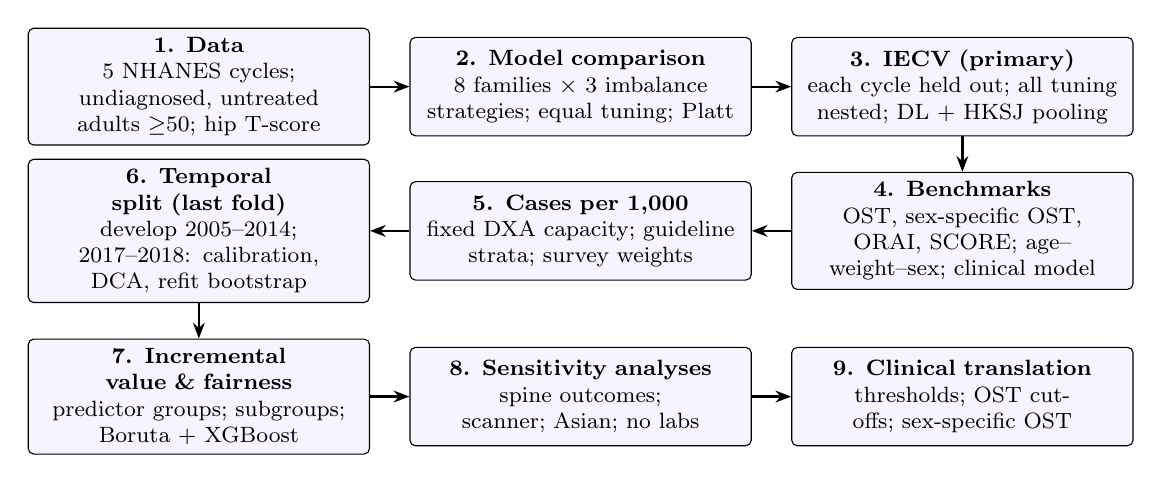
\begin{tikzpicture}[
  st/.style={draw, rounded corners=2pt, align=center, text width=4.1cm, minimum height=1.25cm, font=\footnotesize, fill=blue!4, execute at begin node={\hyphenpenalty=10000}},
  arr/.style={-{Stealth[length=2mm]}, thick},
  node distance=0.45cm and 0.5cm]
\node[st] (s1) {\textbf{1. Data}\\ 5 NHANES cycles; undiagnosed, untreated adults $\ge$50; hip T-score};
\node[st, right=of s1] (s2) {\textbf{2. Model comparison}\\ 8 families $\times$ 3 imbalance strategies; equal tuning; Platt};
\node[st, right=of s2] (s3) {\textbf{3. IECV (primary)}\\ each cycle held out; all tuning nested; DL + HKSJ pooling};
\node[st, below=of s3] (s4) {\textbf{4. Benchmarks}\\ OST, sex-specific OST, ORAI, SCORE; age--weight--sex; clinical model};
\node[st, left=of s4] (s5) {\textbf{5. Cases per 1,000}\\ fixed DXA capacity; guideline strata; survey weights};
\node[st, left=of s5] (s6) {\textbf{6. Temporal split (last fold)}\\ develop 2005--2014; 2017--2018: calibration, DCA, refit bootstrap};
\node[st, below=of s6] (s7) {\textbf{7. Incremental value \& fairness}\\ predictor groups; subgroups; Boruta + XGBoost};
\node[st, right=of s7] (s8) {\textbf{8. Sensitivity analyses}\\ spine outcomes; scanner; Asian; no labs};
\node[st, right=of s8] (s9) {\textbf{9. Clinical translation}\\ thresholds; OST cut-offs; sex-specific OST};
\draw[arr] (s1) -- (s2); \draw[arr] (s2) -- (s3); \draw[arr] (s3) -- (s4);
\draw[arr] (s4) -- (s5); \draw[arr] (s5) -- (s6); \draw[arr] (s6) -- (s7);
\draw[arr] (s7) -- (s8); \draw[arr] (s8) -- (s9);
\end{tikzpicture}
\caption{Study workflow. Imputation, scaling and resampling were fitted inside cross-validation folds. In the temporal split, the 2017--2018 cycle was used only for evaluation; in IECV each cycle was held out in turn.}
\label{fig:workflow}
\end{figure}

{\setlength{\tabcolsep}{4pt}\small
\begin{longtable}{lccc}
\caption{Characteristics of the development (2005--2014) and temporal validation (2017--2018) sets. Mean (SD) or $n$ (\%); unweighted tests.}\label{tab:devval}\\
\toprule
Characteristic & Development ($n=7{,}649$) & Validation ($n=2{,}008$) & $P$ \\
\midrule
\endfirsthead
\toprule
Characteristic & Development & Validation & $P$ \\
\midrule
\endhead
\bottomrule
\endfoot
Osteoporosis (hip) & 343 (4.5) & 96 (4.8) & \\
Age, years & 64.25 (9.48) & 64.07 (8.91) & 0.43 \\
Income-to-poverty ratio & 2.72 (1.62) & 2.69 (1.60) & 0.48 \\
Education level (1--5) & 3.22 (1.34) & 3.48 (1.25) & $<$0.001 \\
BMI, kg/m$^2$ & 28.63 (5.46) & 29.14 (5.94) & $<$0.001 \\
Weight, kg & 80.51 (17.70) & 81.11 (19.22) & 0.21 \\
Height, cm & 167.50 (9.97) & 166.53 (9.81) & $<$0.001 \\
Waist, cm & 100.95 (13.62) & 101.77 (14.39) & 0.022 \\
Calcium, mg/dL & 9.46 (0.38) & 9.32 (0.37) & $<$0.001 \\
Phosphorus, mg/dL & 3.74 (0.56) & 3.54 (0.53) & $<$0.001 \\
Alkaline phosphatase, U/L & 72.64 (24.37) & 82.57 (25.16) & $<$0.001 \\
Creatinine, mg/dL & 0.99 (0.54) & 0.96 (0.41) & 0.031 \\
Albumin, g/dL & 4.20 (0.30) & 4.04 (0.30) & $<$0.001 \\
Uric acid, mg/dL & 5.71 (1.42) & 5.66 (1.47) & 0.21 \\
Glucose, mg/dL & 110.18 (44.03) & 109.68 (43.61) & 0.66 \\
Total protein, g/dL & 7.12 (0.50) & 7.12 (0.44) & 0.67 \\
Cholesterol, mg/dL & 199.23 (43.63) & 192.77 (44.14) & $<$0.001 \\
25(OH) vitamin D, nmol/L & 65.06 (25.99) & 75.84 (32.93) & $<$0.001 \\
Female sex & 3,293 (43.1) & 858 (42.7) & 0.81 \\
Diabetes & 1,380 (18.1) & 468 (23.3) & $<$0.001 \\
Arthritis & 3,027 (39.7) & 816 (40.7) & 0.41 \\
Stroke & 429 (5.6) & 128 (6.4) & 0.22 \\
Coronary heart disease & 570 (7.5) & 156 (7.8) & 0.67 \\
Cancer & 1,181 (15.5) & 305 (15.2) & 0.80 \\
Former smoker & 2,722 (35.6) & 621 (30.9) & $<$0.001 \\
Current smoker & 1,338 (17.5) & 316 (15.7) & 0.067 \\
Prior hip, wrist or spine fracture & 917 (12.0) & 250 (12.5) & 0.59 \\
Parental hip fracture & 716 (9.6) & 218 (11.0) & 0.068 \\
Ever daily glucocorticoid use & 390 (5.1) & 127 (6.4) & 0.032 \\
Postmenopausal & 2,889 (38.5) & 755 (38.6) & 0.95 \\
Ever used female hormones & 1,161 (15.5) & 208 (10.7) & $<$0.001 \\
Alcohol $\ge$3 drinks/day & 168 (2.3) & 57 (3.0) & 0.097 \\
Mexican American & 1,118 (14.6) & 231 (11.5) & $<$0.001 \\
Other Hispanic & 608 (7.9) & 217 (10.8) & $<$0.001 \\
Non-Hispanic Black & 1,549 (20.3) & 485 (24.2) & $<$0.001 \\
Other/multiracial (incl.\ Asian) & 453 (5.9) & 357 (17.8) & $<$0.001 \\
\end{longtable}}

\begin{table}[H]
\centering
\caption{Cross-validated AUROC of each model family before and after equal-budget tuning (Optuna, 40 trials per family, development set, same 5 folds), with its best imbalance strategy. Stacking used the tuned base learners. Changes are computed from unrounded values. The tuning estimate for LR (0.879) is higher than its cross-fitted internal estimate (0.877) because it was obtained on the folds used for tuning. Search spaces and selected values are in Supplementary Table~\ref{tab:hyper}.}
\label{tab:tuned}
\small
\begin{tabular}{llcccc}
\toprule
Family & Strategy & Trials & Default AUROC & Tuned AUROC & Change \\
\midrule
LR & None & 40 & 0.876 & 0.879 & 0.002 \\
SVM & Class wt & 40 & 0.841 & 0.876 & 0.035 \\
LR-spline & None & 40 & 0.873 & 0.875 & 0.001 \\
XGBoost & None & 40 & 0.857 & 0.875 & 0.018 \\
LightGBM & None & 40 & 0.852 & 0.875 & 0.023 \\
Stacking & Class wt & -- & 0.865 & 0.874 & 0.010 \\
CatBoost & None & 40 & 0.865 & 0.873 & 0.008 \\
RF & Class wt & 40 & 0.861 & 0.864 & 0.003 \\
\bottomrule
\end{tabular}
\end{table}

\begin{table}[H]
\centering
\caption{Clinical model (19 predictors from history and examination; no laboratory tests, race/ethnicity, income or education) in internal--external cross-validation, with the penalty $C$ re-tuned within the four development cycles. $\Delta$, AUROC differences with 95\% CIs (paired bootstrap per cycle; DerSimonian--Laird with HKSJ CIs when pooled). The pooled AUROC is meta-analysed across cycles; Supplementary Table~\ref{tab:casesstrata} instead pools the out-of-cycle predictions (0.865).}
\label{tab:iecvclin}
\footnotesize
\setlength{\tabcolsep}{3pt}
\resizebox{\textwidth}{!}{%
\begin{tabular}{lcccccc}
\toprule
Held-out cycle & $C$ & AUROC & Slope & $\Delta$ vs OST & $\Delta$ vs age, weight, sex & Full model minus clinical \\
\midrule
2005--2006 & 31.7 & 0.900 & 1.08 & 0.000 ($-$0.026 to 0.027) & $-$0.010 ($-$0.030 to 0.010) & 0.012 (0.002 to 0.022) \\
2007--2008 & 0.26 & 0.897 & 1.26 & 0.030 (0.012 to 0.049) & 0.025 (0.009 to 0.040) & 0.003 ($-$0.011 to 0.018) \\
2009--2010 & 1.00 & 0.872 & 0.95 & 0.014 ($-$0.001 to 0.029) & 0.019 (0.006 to 0.032) & 0.005 ($-$0.008 to 0.018) \\
2013--2014 & 0.13 & 0.820 & 0.73 & 0.012 ($-$0.011 to 0.035) & 0.008 ($-$0.011 to 0.028) & 0.021 (0.008 to 0.035) \\
2017--2018 & 0.20 & 0.859 & 1.00 & 0.018 ($-$0.001 to 0.037) & 0.008 ($-$0.008 to 0.024) & 0.010 ($-$0.001 to 0.021) \\
\midrule
Pooled (HKSJ) & -- & 0.871 (0.831--0.910) & -- & 0.016 (0.004 to 0.029) & 0.011 ($-$0.005 to 0.027) & 0.011 (0.003 to 0.019) \\
\bottomrule
\end{tabular}}
\end{table}

\begin{table}[H]
\centering
\caption{Tuned ML families in internal--external cross-validation with fully nested tuning: for each held-out cycle, every family re-selected its imbalance strategy and was re-tuned (40 Optuna trials, same search spaces) on the other four cycles only, as was the penalty of the full model; stacking omitted. AUROC by held-out cycle and pooled (random effects); $\Delta$, family minus full model, pooled with 90\% HKSJ CI; equivalent if within $\pm$0.02. The last column gives $\Delta$ when hyperparameters were instead fixed at their 2005--2014 values, which overlap four held-out cycles. Strategies selected: none for LR-spline, XGBoost and CatBoost; class weighting for SVM and RF; none for LightGBM except class weighting when 2013--2014 was held out.}
\label{tab:iecvml}
\footnotesize
\resizebox{\textwidth}{!}{%
\begin{tabular}{lccccccclc}
\toprule
 & & \multicolumn{5}{c}{Held-out cycle} & \multicolumn{2}{c}{Nested tuning} & Fixed hyperparameters \\
\cmidrule(lr){3-7}\cmidrule(lr){8-9}\cmidrule(lr){10-10}
Family & Pooled & 2005--06 & 2007--08 & 2009--10 & 2013--14 & 2017--18 & $\Delta$ vs full model (90\% CI) & Equivalent & $\Delta$ (90\% CI) \\
\midrule
Full model (LR, re-tuned) & 0.881 & 0.912 & 0.901 & 0.877 & 0.841 & 0.869 & -- & -- & -- \\
LR-spline & 0.879 & 0.908 & 0.892 & 0.884 & 0.839 & 0.869 & $-$0.003 ($-$0.008 to 0.003) & Yes & 0.000 ($-$0.006 to 0.006) \\
SVM & 0.878 & 0.912 & 0.896 & 0.874 & 0.834 & 0.870 & $-$0.003 ($-$0.007 to 0.001) & Yes & 0.000 ($-$0.004 to 0.004) \\
RF & 0.870 & 0.914 & 0.894 & 0.861 & 0.812 & 0.862 & $-$0.010 ($-$0.021 to 0.000) & No & $-$0.013 ($-$0.025 to $-$0.001) \\
XGBoost & 0.878 & 0.912 & 0.895 & 0.874 & 0.836 & 0.868 & $-$0.003 ($-$0.010 to 0.003) & Yes & $-$0.003 ($-$0.009 to 0.004) \\
LightGBM & 0.875 & 0.914 & 0.892 & 0.869 & 0.825 & 0.867 & $-$0.006 ($-$0.012 to 0.001) & Yes & $-$0.003 ($-$0.009 to 0.004) \\
CatBoost & 0.879 & 0.919 & 0.896 & 0.880 & 0.827 & 0.867 & $-$0.002 ($-$0.009 to 0.005) & Yes & $-$0.002 ($-$0.010 to 0.005) \\
\bottomrule
\end{tabular}}
\end{table}

\begin{table}[H]
\centering
\caption{Sex-specific OST and all tools by sex (temporal validation set). The sex-specific OST is a logistic model of OST, sex and their interaction fitted on the development set: logit risk $=-3.195-0.353\,\text{OST}+0.601\,\text{female}-0.070\,\text{OST}\times\text{female}$. Within each sex it ranks people as OST does, so its sex-specific AUROC equals that of OST. $\Delta$, full model minus each tool (paired bootstrap 95\% CI).}
\label{tab:ostsexspec}
\footnotesize
\setlength{\tabcolsep}{3pt}
\resizebox{\textwidth}{!}{%
\begin{tabular}{lcccccc}
\toprule
 & Full model & Age, weight, sex & OST, sex-specific & OST & SCORE & ORAI \\
\midrule
\multicolumn{7}{l}{\textit{All participants ($n=2{,}008$; 96 cases)}} \\
AUROC (95\% CI) & 0.869 (0.831--0.904) & 0.851 (0.808--0.890) & 0.850 (0.806--0.890) & 0.841 (0.796--0.883) & 0.841 (0.799--0.879) & 0.791 (0.742--0.834) \\
Tool minus sex-specific OST & 0.019 ($-$0.0004 to 0.041) & 0.001 ($-$0.002 to 0.005) & -- & $-$0.009 ($-$0.017 to $-$0.002) & $-$0.010 ($-$0.034 to 0.016) & $-$0.059 ($-$0.090 to $-$0.032) \\
Detected / referred at Youden threshold & 77 / 23.8\% & 75 / 24.4\% & 76 / 25.3\% & 79 / 30.9\% & 80 / 30.2\% & 72 / 28.8\% \\
\addlinespace
\multicolumn{7}{l}{\textit{Women ($n=858$; 72 cases)}} \\
AUROC & 0.853 & 0.834 & 0.834 & 0.834 & 0.843 & 0.802 \\
$\Delta$ full model (95\% CI) & -- & 0.019 ($-$0.005 to 0.047) & & 0.019 ($-$0.005 to 0.046) & 0.011 ($-$0.020 to 0.042) & 0.051 (0.021--0.086) \\
\addlinespace
\multicolumn{7}{l}{\textit{Men ($n=1{,}150$; 24 cases)}} \\
AUROC & 0.820 & 0.800 & 0.800 & 0.800 & 0.806 & 0.779 \\
$\Delta$ full model (95\% CI) & -- & 0.021 ($-$0.030 to 0.069) & & 0.020 ($-$0.031 to 0.068) & 0.014 ($-$0.038 to 0.068) & 0.042 ($-$0.027 to 0.120) \\
\bottomrule
\end{tabular}}
\end{table}

\begin{table}[H]
\centering
\caption{Incremental value of predictor groups in nested logistic models. CV, 5-fold cross-validation in the development set; temporal, 2017--2018 validation set. $\Delta$AUROC compares each model with the previous row (paired bootstrap 95\% CI and $P$).}
\label{tab:incr}
\footnotesize
\setlength{\tabcolsep}{4pt}
\resizebox{\textwidth}{!}{%
\begin{tabular}{lcccccc}
\toprule
Predictors & $k$ & CV AUROC & Temporal AUROC (95\% CI) & AUPRC & $\Delta$AUROC (95\% CI) & $P$ \\
\midrule
Age, weight, sex & 3 & 0.856 & 0.851 (0.808--0.890) & 0.312 & -- & -- \\
+ other body measures, socio-demographics & 8 & 0.864 & 0.858 (0.816--0.894) & 0.332 & 0.007 ($-$0.005 to 0.018) & 0.21 \\
+ clinical risk factors and history & 21 & 0.869 & 0.859 (0.819--0.894) & 0.318 & 0.001 ($-$0.010 to 0.012) & 0.85 \\
+ laboratory tests & 31 & 0.872 & 0.863 (0.825--0.898) & 0.325 & 0.005 ($-$0.002 to 0.011) & 0.17 \\
+ race/ethnicity & 35 & 0.877 & 0.869 (0.831--0.904) & 0.335 & 0.006 ($-$0.001 to 0.012) & 0.14 \\
\bottomrule
\end{tabular}}
\end{table}

\begin{table}[H]
\centering
\caption{Temporal validation performance of every model, including operating characteristics ($n=2{,}008$; 96 with osteoporosis), with 95\% bootstrap CIs. Sensitivity, specificity and the proportion referred are at each model's development-set Youden threshold; for OST, ORAI and SCORE, values other than AUROC and AUPRC are for the recalibrated score. All ML families were tuned with the same budget. $\Delta$AUROC, full model minus each alternative (paired bootstrap; 95\% percentile CI, except 90\% CI for the equivalence family); $P$, two-sided bootstrap $P$; $P_{\text{Holm}}$, Holm-adjusted within its family. Equivalence margin $\pm$0.02.}
\label{tab:perffull}
\footnotesize
\setlength{\tabcolsep}{3pt}
\resizebox{\textwidth}{!}{%
\begin{tabular}{lcccccccccc}
\toprule
Model & AUROC (95\% CI) & AUPRC & Brier & Sens. & Spec. & Referred & Slope (95\% CI) & $\Delta$AUROC (95\% CI) & $P$ & $P_{\text{Holm}}$ \\
\midrule
\textbf{Full model (LR, 35 predictors)} & \textbf{0.869 (0.831--0.904)} & \textbf{0.335} & \textbf{0.038} & \textbf{0.802} & \textbf{0.791} & \textbf{23.8\%} & \textbf{1.00 (0.85--1.18)} & -- & -- & -- \\
\addlinespace\multicolumn{11}{l}{\textit{Primary comparison}} \\
OST & 0.841 (0.796--0.883) & 0.280 & 0.040 & 0.823 & 0.717 & 30.9\% & 0.98 (0.79--1.20) & 0.028 (0.007--0.052) & 0.014 & -- \\
\addlinespace\multicolumn{11}{l}{\textit{Secondary comparisons (Holm-adjusted, family of four)}} \\
LR: age, weight, sex & 0.851 (0.808--0.890) & 0.312 & 0.039 & 0.781 & 0.783 & 24.4\% & 1.04 (0.86--1.28) & 0.018 ($-$0.001 to 0.039) & 0.070 & 0.14 \\
SCORE & 0.841 (0.799--0.879) & 0.263 & 0.040 & 0.833 & 0.725 & 30.2\% & 1.04 (0.87--1.25) & 0.029 (0.003--0.055) & 0.028 & 0.084 \\
ORAI & 0.791 (0.742--0.834) & 0.177 & 0.042 & 0.750 & 0.735 & 28.8\% & 0.93 (0.75--1.11) & 0.078 (0.047--0.115) & 0.001 & 0.004 \\
Boruta + XGBoost pipeline & 0.856 (0.820--0.892) & 0.295 & 0.039 & 0.844 & 0.680 & 34.5\% & 1.04 (0.89--1.24) & 0.013 ($-$0.007 to 0.030) & 0.18 & 0.18 \\
\addlinespace\multicolumn{11}{l}{\textit{Tuned ML families vs LR: equivalence (90\% CI, margin $\pm$0.02; no multiplicity adjustment)}} \\
LR-spline & 0.869 (0.832--0.903) & 0.320 & 0.038 & 0.802 & 0.793 & 23.6\% & 1.06 (0.91--1.25) & 0.000 ($-$0.008 to 0.007) & 0.94 & -- \\
SVM & 0.870 (0.832--0.906) & 0.367 & 0.037 & 0.740 & 0.835 & 19.2\% & 1.03 (0.87--1.22) & $-$0.001 ($-$0.010 to 0.009) & 0.87 & -- \\
Random forest & 0.862 (0.823--0.900) & 0.313 & 0.038 & 0.812 & 0.742 & 28.4\% & 1.04 (0.87--1.24) & 0.007 ($-$0.008 to 0.020) & 0.40 & -- \\
XGBoost & 0.868 (0.834--0.901) & 0.320 & 0.038 & 0.771 & 0.828 & 20.0\% & 1.04 (0.90--1.22) & 0.001 ($-$0.010 to 0.012) & 0.88 & -- \\
LightGBM & 0.867 (0.832--0.902) & 0.325 & 0.038 & 0.802 & 0.745 & 28.1\% & 1.06 (0.92--1.26) & 0.002 ($-$0.010 to 0.012) & 0.83 & -- \\
CatBoost & 0.867 (0.830--0.905) & 0.333 & 0.038 & 0.823 & 0.741 & 28.6\% & 1.07 (0.92--1.26) & 0.002 ($-$0.011 to 0.013) & 0.86 & -- \\
Stacking & 0.872 (0.836--0.908) & 0.338 & 0.038 & 0.812 & 0.769 & 25.8\% & 1.04 (0.89--1.24) & $-$0.003 ($-$0.012 to 0.006) & 0.51 & -- \\
\addlinespace\multicolumn{11}{l}{\textit{Exploratory (not part of a comparison family)}} \\
Full model without race & 0.863 (0.825--0.898) & 0.325 & 0.038 & 0.792 & 0.798 & 23.1\% & 1.00 (0.84--1.19) & 0.006 ($-$0.001 to 0.012) & 0.14 & -- \\
Short form (10 predictors, no blood test) & 0.852 (0.810--0.887) & 0.310 & 0.039 & 0.812 & 0.751 & 27.6\% & 0.96 (0.80--1.17) & 0.018 (0.003--0.033) & 0.018 & -- \\
\bottomrule
\end{tabular}}
\end{table}

\begin{table}[H]
\centering
\caption{Guideline strata, the population not routinely screened, and survey weighting, from the pooled out-of-cycle predictions of the internal--external cross-validation. AUROCs pool the out-of-cycle predictions of all cycles (one-stage), so they differ slightly from the meta-analysed estimates in Table~\ref{tab:iecv} and Supplementary Table~\ref{tab:iecvclin}. AUROC difference, full model minus OST (bootstrap within cycles). Cases per 1,000 at a referral rate of 20\% within each population (random tie-breaking); $\Delta$, full model minus OST (95\% CI). Weighted rows use the examination weights (divided by five when pooled); referral is the top 20\% of the weighted population, and CIs are from a simple bootstrap within cycles, not a design-based bootstrap.}
\label{tab:casesstrata}
\footnotesize
\setlength{\tabcolsep}{3pt}
\resizebox{\textwidth}{!}{%
\begin{tabular}{lrrcccccccc}
\toprule
 & & & \multicolumn{3}{c}{AUROC} & & \multicolumn{4}{c}{Cases per 1,000 at 20\% referral} \\
\cmidrule(lr){4-6}\cmidrule(lr){8-11}
Population & $n$ & Cases & Full & Clinical & OST & $\Delta$AUROC (95\% CI) & Total & Full & OST & $\Delta$ (95\% CI) \\
\midrule
All participants & 9,657 & 439 & 0.875 & 0.865 & 0.850 & 0.026 (0.015--0.036) & 45.5 & 35.3 & 32.5 & 2.8 (1.0--4.3) \\
Not routinely screened (all but women $\ge$65) & 7,954 & 216 & 0.848 & 0.833 & 0.819 & 0.029 (0.012--0.046) & 27.2 & 20.7 & 18.5 & 2.3 (0.9--3.9) \\
Women 50--64 & 2,448 & 95 & 0.869 & 0.858 & 0.838 & 0.031 (0.009--0.054) & 38.8 & 27.8 & 27.2 & 0.6 ($-$2.9 to 4.1) \\
Women $\ge$65 & 1,703 & 223 & 0.824 & 0.814 & 0.795 & 0.029 (0.009--0.048) & 130.9 & 75.7 & 72.4 & 3.4 ($-$4.1 to 10.0) \\
Men 50--69 & 3,699 & 45 & 0.797 & 0.771 & 0.772 & 0.025 ($-$0.024 to 0.078) & 12.2 & 7.8 & 8.1 & $-$0.3 ($-$1.4 to 1.1) \\
Men $\ge$70 & 1,807 & 76 & 0.778 & 0.758 & 0.759 & 0.019 ($-$0.015 to 0.056) & 42.1 & 27.1 & 24.9 & 2.2 ($-$2.8 to 6.6) \\
\addlinespace
All cycles, survey-weighted & 9,657 & 439 & & & & & 38.9 & 30.9 & 28.4 & 2.4 (0.5--4.5) \\
2017--2018, unweighted & 2,008 & 96 & & & & & 47.8 & 36.9 & 34.9 & 2.0 ($-$1.5 to 5.0) \\
2017--2018, survey-weighted & 2,008 & 96 & & & & & 41.6 & 34.6 & 30.5 & 4.1 ($-$0.7 to 9.8) \\
\bottomrule
\end{tabular}}
\end{table}

\begin{table}[H]
\centering
\caption{OST at its published cut-offs (no fitting) versus the full model at a threshold referring the same proportion of participants (temporal validation set, 96 cases). Additional cases: full model minus OST, with 95\% bootstrap CI.}
\label{tab:ost}
\small
\begin{tabular}{llcccc}
\toprule
Referral rate & Rule & Cases detected & Sensitivity & Specificity & Additional cases \\
\midrule
39.1\% & OST $<2$ & 83 & 0.865 & 0.633 & \\
 & Full model & 86 & 0.896 & 0.634 & 3 ($-$2 to 8) \\
\addlinespace
14.9\% & OST $<-1$ & 62 & 0.646 & 0.876 & \\
 & Full model & 68 & 0.708 & 0.879 & 6 ($-$2 to 14) \\
\bottomrule
\end{tabular}
\end{table}

\begin{table}[H]
\centering
\caption{Net benefit in the temporal validation set at selected threshold probabilities within the 2\%--15\% range (95\% bootstrap CIs), with true and false positives per 100 people screened. OST, ORAI and SCORE recalibrated to probabilities. Every model had higher net benefit than referring everyone or no one at every threshold from 2\% to 15\%.}
\label{tab:nb}
\small
\begin{tabular}{llccc}
\toprule
Model & Threshold & Net benefit (95\% CI) & TP per 100 & FP per 100 \\
\midrule
Full model & 0.05 & 0.0279 (0.0194--0.0371) & 3.78 & 18.97 \\
 & 0.10 & 0.0215 (0.0148--0.0299) & 3.14 & 8.86 \\
 & 0.15 & 0.0122 (0.0059--0.0191) & 2.19 & 5.48 \\
\addlinespace
Boruta + XGBoost & 0.05 & 0.0259 (0.0176--0.0341) & 3.64 & 19.92 \\
 & 0.10 & 0.0190 (0.0122--0.0268) & 2.89 & 8.91 \\
 & 0.15 & 0.0146 (0.0071--0.0220) & 2.44 & 5.53 \\
\addlinespace
LR: age, weight, sex & 0.05 & 0.0265 (0.0181--0.0354) & 3.69 & 19.62 \\
 & 0.10 & 0.0181 (0.0106--0.0256) & 2.84 & 9.26 \\
 & 0.15 & 0.0114 (0.0056--0.0178) & 1.89 & 4.28 \\
\addlinespace
OST (recalibrated) & 0.05 & 0.0268 (0.0181--0.0356) & 3.74 & 20.12 \\
 & 0.10 & 0.0183 (0.0108--0.0261) & 2.84 & 9.11 \\
 & 0.15 & 0.0077 (0.0021--0.0140) & 1.69 & 5.23 \\
\addlinespace
ORAI (recalibrated) & 0.05 & 0.0202 (0.0128--0.0280) & 3.09 & 20.27 \\
 & 0.10 & 0.0122 (0.0064--0.0188) & 1.99 & 6.97 \\
 & 0.15 & 0.0048 (0.0011--0.0091) & 0.80 & 1.79 \\
\addlinespace
SCORE (recalibrated) & 0.05 & 0.0257 (0.0177--0.0345) & 3.64 & 20.22 \\
 & 0.10 & 0.0160 (0.0091--0.0231) & 2.59 & 8.91 \\
 & 0.15 & 0.0085 (0.0031--0.0144) & 1.64 & 4.48 \\
\bottomrule
\end{tabular}
\end{table}

\begin{table}[H]
\centering
\caption{Sensitivity of survey-weighted estimates to the weights (temporal validation set). The non-response factor (inverse of the modelled probability of a valid DXA result) had a median of 1.17, a 99th percentile of 3.85 and a maximum of 32.5 (18 participants above 5, 11 above 10). Normalised non-response-adjusted weights ranged from 0.13 (1st percentile) to 6.67 (99th percentile), maximum 10.1; the Kish design effect due to weighting was 2.87 with examination weights and 2.84 with adjusted weights. Weighted AUROCs; point estimates. $\Delta$ is computed from unrounded AUROCs, so it may differ by 0.001 from the difference of the rounded values.}
\label{tab:wtrim}
\footnotesize
\resizebox{\textwidth}{!}{%
\begin{tabular}{lcccccc}
\toprule
Weights & Observed prev. & Predicted prev. (full model) & Full model & Age, weight, sex & OST & $\Delta$ vs OST \\
\midrule
Examination weight & 4.2\% & 4.1\% & 0.889 & 0.870 & 0.868 & 0.020 \\
Non-response adjusted & 4.2\% & 3.9\% & 0.872 & 0.856 & 0.849 & 0.023 \\
Adjusted, trimmed at 99th percentile & 4.2\% & 4.0\% & 0.871 & 0.855 & 0.848 & 0.023 \\
Adjusted, trimmed at 5 $\times$ median & 4.7\% & 4.4\% & 0.870 & 0.851 & 0.845 & 0.025 \\
Adjusted, factor capped at 3 & 4.1\% & 4.0\% & 0.888 & 0.869 & 0.867 & 0.021 \\
\bottomrule
\end{tabular}}
\end{table}

\begin{table}[H]
\centering
\caption{Performance of the full model by subgroup in the temporal validation set, at the global threshold (4.8\%). Pred., mean predicted risk. 95\% bootstrap CIs. The last three columns show the race-free model at its own threshold (5.2\%). In the models, non-Hispanic Asian adults are part of the other/multiracial category (see Methods). $^a$All 6 cases were detected, so every bootstrap resample gave a sensitivity of 1.000 and the percentile interval is degenerate; it does not indicate certainty.}
\label{tab:fair}
\footnotesize
\setlength{\tabcolsep}{3pt}
\resizebox{\textwidth}{!}{%
\begin{tabular}{lrrcccccccc}
\toprule
 & & & & \multicolumn{4}{c}{Full model} & \multicolumn{3}{c}{Race-free model} \\
\cmidrule(lr){5-8}\cmidrule(lr){9-11}
Subgroup & $n$ & Cases & Prev. & Pred. & AUROC (95\% CI) & Detected, sensitivity (95\% CI) & Spec. & Pred. & AUROC & Sens. \\
\midrule
Women & 858 & 72 & 8.4\% & 7.2\% & 0.853 (0.811--0.894) & 61/72, 0.847 (0.754--0.922) & 0.669 & 7.3\% & 0.847 & 0.847 \\
Men & 1,150 & 24 & 2.1\% & 2.4\% & 0.820 (0.733--0.899) & 16/24, 0.667 (0.468--0.850) & 0.876 & 2.5\% & 0.816 & 0.625 \\
\addlinespace
Age 50--64 & 1,157 & 32 & 2.8\% & 2.7\% & 0.861 (0.790--0.924) & 21/32, 0.656 (0.500--0.818) & 0.864 & 2.7\% & 0.849 & 0.625 \\
Age 65--79 & 651 & 35 & 5.4\% & 5.0\% & 0.855 (0.787--0.912) & 29/35, 0.829 (0.696--0.944) & 0.752 & 5.2\% & 0.847 & 0.829 \\
Age $\ge$80 & 200 & 29 & 14.5\% & 12.9\% & 0.793 (0.696--0.882) & 27/29, 0.931 (0.833--1.000) & 0.450 & 13.0\% & 0.800 & 0.931 \\
\addlinespace
Non-Hispanic white & 718 & 51 & 7.1\% & 6.3\% & 0.851 (0.799--0.897) & 42/51, 0.824 (0.717--0.917) & 0.736 & 5.5\% & 0.855 & 0.804 \\
Non-Hispanic Black & 485 & 7 & 1.4\% & 2.1\% & 0.782 (0.570--0.930) & 4/7, 0.571 (0.143--1.000) & 0.874 & 3.2\% & 0.776 & 0.571 \\
Mexican American & 231 & 8 & 3.5\% & 2.7\% & 0.816 (0.674--0.956) & 4/8, 0.500 (0.143--0.889) & 0.883 & 3.7\% & 0.803 & 0.625 \\
Other Hispanic & 217 & 6 & 2.8\% & 3.8\% & 0.963 (0.930--0.987) & 6/6, 1.000 (1.000--1.000)$^a$ & 0.806 & 3.8\% & 0.957 & 1.000 \\
Non-Hispanic Asian & 275 & 20 & 7.3\% & 6.0\% & 0.904 (0.840--0.953) & 18/20, 0.900 (0.750--1.000) & 0.698 & 5.8\% & 0.904 & 0.850 \\
Other/multiracial (non-Asian) & 82 & 4 & 4.9\% & 3.9\% & 0.821 (0.450--0.988) & 3/4, 0.750 (0.000--1.000) & 0.744 & 3.8\% & 0.814 & 0.750 \\
\bottomrule
\end{tabular}}
\end{table}

\begin{table}[H]
\centering
\caption{Sensitivity analyses: temporal-validation AUROC and calibration slope.}
\label{tab:sens}
\small
\begin{tabular}{lcccc}
\toprule
Analysis / model & Dev. prev. & Val. prev. & AUROC & Slope \\
\midrule
\multicolumn{5}{l}{\textit{Hip or complete-scan lumbar spine (L1--L4)}} \\
\quad Full model & 7.2\% & 6.7\% & 0.846 & 1.06 \\
\quad OST &  &  & 0.823 & 1.11 \\
\quad LR: age, weight, sex &  &  & 0.836 & 1.12 \\
\multicolumn{5}{l}{\textit{Hip or lumbar spine from $\ge$2 valid vertebrae}} \\
\quad Full model & 8.4\% & 8.2\% & 0.840 & 1.05 \\
\quad OST &  &  & 0.801 & 1.04 \\
\quad LR: age, weight, sex &  &  & 0.824 & 1.10 \\
\multicolumn{5}{l}{\textit{Excluding non-Hispanic Asian participants}} \\
\quad Full model & 4.4\% & 4.4\% & 0.861 & 0.92 \\
\multicolumn{5}{l}{\textit{Development on 2013--2014 only (same scanner type)}} \\
\quad Full model & 4.8\% & 4.8\% & 0.854 & 1.13 \\
\multicolumn{5}{l}{\textit{Development set without 2005--2006}} \\
\quad Full model & 4.5\% & 4.8\% & 0.869 & 1.00 \\
\multicolumn{5}{l}{\textit{Without laboratory predictors}} \\
\quad Full model & 4.5\% & 4.8\% & 0.863 & 0.98 \\
\multicolumn{5}{l}{\textit{Without alcohol predictor}} \\
\quad Full model & 4.5\% & 4.8\% & 0.869 & 0.99 \\
\multicolumn{5}{l}{\textit{Including previously diagnosed or treated participants}} \\
\quad Full model & 6.4\% & 7.1\% & 0.859 & 0.97 \\
\quad OST &  &  & 0.824 & 0.89 \\
\quad LR: age, weight, sex &  &  & 0.839 & 0.95 \\
\bottomrule
\end{tabular}
\end{table}

\begin{table}[H]
\centering
\caption{Sensitivity to a possible scanner offset. Hip T-scores of one scanner period were shifted by 0.15 reference SD (the observed difference in mean femoral neck BMD in women), the outcome was redefined and all models were refitted on the development set.}
\label{tab:scanner}
\footnotesize
\begin{tabular}{llcccc}
\toprule
Scenario & Model & Dev. prev. & Val. prev. & AUROC & Slope \\
\midrule
Pre-2013 T-scores lowered by 0.15 SD & Full model & 5.5\% & 4.8\% & 0.871 & 1.01 \\
 & Age, weight, sex & & & 0.851 & 1.08 \\
 & OST & & & 0.841 & 1.02 \\
\addlinespace
2013--2018 T-scores raised by 0.15 SD & Full model & 4.1\% & 3.5\% & 0.885 & 1.07 \\
 & Age, weight, sex & & & 0.859 & 1.07 \\
 & OST & & & 0.849 & 1.00 \\
\bottomrule
\end{tabular}
\end{table}

\begin{table}[H]
\centering
\caption{Re-implementation of the published analysis: 10-fold cross-validation in the development set (mean $\pm$ SD across folds). Features were selected once on the full development set, so these estimates are optimistic.}
\label{tab:reimpl}
\small
\begin{tabular}{llcc}
\toprule
Feature selection & Classifier & AUROC & Accuracy \\
\midrule
Boruta & LR & 0.871 $\pm$ 0.021 & 0.956 \\
 & SVM & 0.657 $\pm$ 0.050 & 0.955 \\
 & RF & 0.849 $\pm$ 0.020 & 0.956 \\
 & XGBoost & 0.845 $\pm$ 0.019 & 0.954 \\
\addlinespace
Lasso & LR & 0.879 $\pm$ 0.020 & 0.957 \\
 & SVM & 0.777 $\pm$ 0.042 & 0.955 \\
 & RF & 0.848 $\pm$ 0.020 & 0.956 \\
 & XGBoost & 0.855 $\pm$ 0.016 & 0.956 \\
\addlinespace
XGBoost importance & LR & 0.872 $\pm$ 0.017 & 0.956 \\
 & SVM & 0.653 $\pm$ 0.086 & 0.956 \\
 & RF & 0.854 $\pm$ 0.025 & 0.956 \\
 & XGBoost & 0.852 $\pm$ 0.022 & 0.955 \\
\bottomrule
\end{tabular}
\end{table}

\begin{table}[H]
\centering
\caption{Full model at alternative operating points in the temporal validation set (96 cases). The first two thresholds were chosen on the development set; the others are fixed predicted risks.}
\label{tab:ops}
\small
\setlength{\tabcolsep}{4pt}
\begin{tabular}{lccccccc}
\toprule
Operating point & Threshold & Referred & Detected & Sens. & Spec. & PPV & NPV \\
\midrule
Youden (development) & 4.8\% & 23.8\% & 77/96 & 0.802 & 0.791 & 0.161 & 0.988 \\
Sensitivity 0.90 in development & 2.3\% & 39.3\% & 86/96 & 0.896 & 0.632 & 0.109 & 0.992 \\
Fixed 3\% & 3.0\% & 32.8\% & 83/96 & 0.865 & 0.699 & 0.126 & 0.990 \\
Fixed 5\% & 5.0\% & 22.8\% & 76/96 & 0.792 & 0.801 & 0.166 & 0.987 \\
Fixed 10\% & 10.0\% & 12.0\% & 63/96 & 0.656 & 0.907 & 0.261 & 0.981 \\
\bottomrule
\end{tabular}
\end{table}

\begin{longtable}{lrr}
\caption{Coefficients of the full model (penalised logistic regression on 35 predictors, recalibrated, original units). Units as in Supplementary Table~\ref{tab:devval}; binary predictors 1 = yes. Coefficients are penalised and correlated predictors are not individually interpretable.}\label{tab:coef}\\
\toprule
Term & Coefficient & Odds ratio per unit \\
\midrule
\endfirsthead
\toprule
Term & Coefficient & Odds ratio per unit \\
\midrule
\endhead
\bottomrule
\endfoot
Intercept & 6.95527 &  \\
Age, years & 0.05908 & 1.061 \\
Income-to-poverty ratio & $-$0.14411 & 0.866 \\
Education level (1--5) & 0.03807 & 1.039 \\
BMI, kg/m$^2$ & $-$0.15810 & 0.854 \\
Weight, kg & $-$0.03937 & 0.961 \\
Height, cm & $-$0.04479 & 0.956 \\
Waist, cm & 0.02589 & 1.026 \\
Calcium, mg/dL & $-$0.01321 & 0.987 \\
Phosphorus, mg/dL & $-$0.00500 & 0.995 \\
Alkaline phosphatase, U/L & 0.00771 & 1.008 \\
Creatinine, mg/dL & 0.29171 & 1.339 \\
Albumin, g/dL & $-$0.27440 & 0.760 \\
Uric acid, mg/dL & $-$0.02154 & 0.979 \\
Glucose, mg/dL & $-$0.00101 & 0.999 \\
Total protein, g/dL & $-$0.20078 & 0.818 \\
Cholesterol, mg/dL & 0.00119 & 1.001 \\
25(OH) vitamin D, nmol/L & $-$0.00539 & 0.995 \\
Female sex & $-$0.02615 & 0.974 \\
Diabetes & 0.18337 & 1.201 \\
Arthritis & $-$0.24444 & 0.783 \\
Stroke & 0.53830 & 1.713 \\
Coronary heart disease & 0.31449 & 1.370 \\
Cancer & $-$0.38293 & 0.682 \\
Former smoker & $-$0.05355 & 0.948 \\
Current smoker & 0.20477 & 1.227 \\
Prior hip, wrist or spine fracture & 0.93243 & 2.541 \\
Parental hip fracture & $-$0.14696 & 0.863 \\
Ever daily glucocorticoid use & 0.14705 & 1.158 \\
Postmenopausal & 0.99824 & 2.714 \\
Ever used female hormones & $-$0.79702 & 0.451 \\
Alcohol $\ge$3 drinks/day & $-$0.33579 & 0.715 \\
Mexican American & $-$0.77710 & 0.460 \\
Other Hispanic & $-$0.36512 & 0.694 \\
Non-Hispanic Black & $-$0.80116 & 0.449 \\
Other/multiracial (incl.\ Asian) & $-$0.26758 & 0.765 \\
\end{longtable}

\begin{table}[H]
\centering
\caption{Model card for the full model (penalised logistic regression).}
\label{tab:modelcard}
\small
\begin{tabular}{p{3.4cm}p{11.6cm}}
\toprule
Item & Description \\
\midrule
Intended use & Ranking adults aged $\ge$50 years who have neither been diagnosed with nor treated for osteoporosis, to prioritise DXA referral when capacity is limited. Not for fracture prediction, treatment decisions, or people already diagnosed or treated. \\
Output & Recalibrated probability of hip osteoporosis (femoral neck or total hip T-score $\le -2.5$). \\
Inputs & 35 predictors: age, sex, race/ethnicity, education, income-to-poverty ratio, body measures, ten serum tests, FRAX-type risk factors, menopause, hormone use and common diagnoses (Methods). A 19-item clinical version omits laboratory tests, race/ethnicity, income and education. \\
Development data & NHANES 2005--2018, five cycles, 9,657 participants, 439 cases; US civilian non-institutionalised population. \\
Validation & Internal--external cross-validation across cycles with nested tuning; 2017--2018 as the last fold. \\
Performance & Pooled AUROC 0.881 (OST 0.856); 2017--2018 AUROC 0.869, calibration slope 1.00, Brier score 0.038; 2.8 more cases per 1,000 screened than OST at 20\% referral. AUROC 0.853 in women and 0.820 in men (2017--2018). \\
Calibration across cycles & Observed-to-expected ratio 0.84--1.16 and slope 0.82--1.25 across held-out cycles; recalibrate the intercept locally before use. \\
Known limitations & Cross-sectional outcome; few cases in men, younger women and minority groups; scanner and laboratory changes between cycles; inputs such as income and vitamin D are rarely available in routine records; no external validation. \\
Simpler alternatives & OST, a sex-specific OST or an age--weight--sex model, which lose about 3 cases per 1,000 screened at the same DXA capacity. \\
Monitoring & Track referral rate, cases detected per scan and observed-to-expected ratio after deployment; refit if calibration drifts. \\
Availability & Coefficients in Supplementary Table~\ref{tab:coef}; code at \url{https://github.com/slxnjdhv/osteoporosis-nhanes}. \\
\bottomrule
\end{tabular}
\end{table}
{\small
}

\begin{figure}[H]
\centering
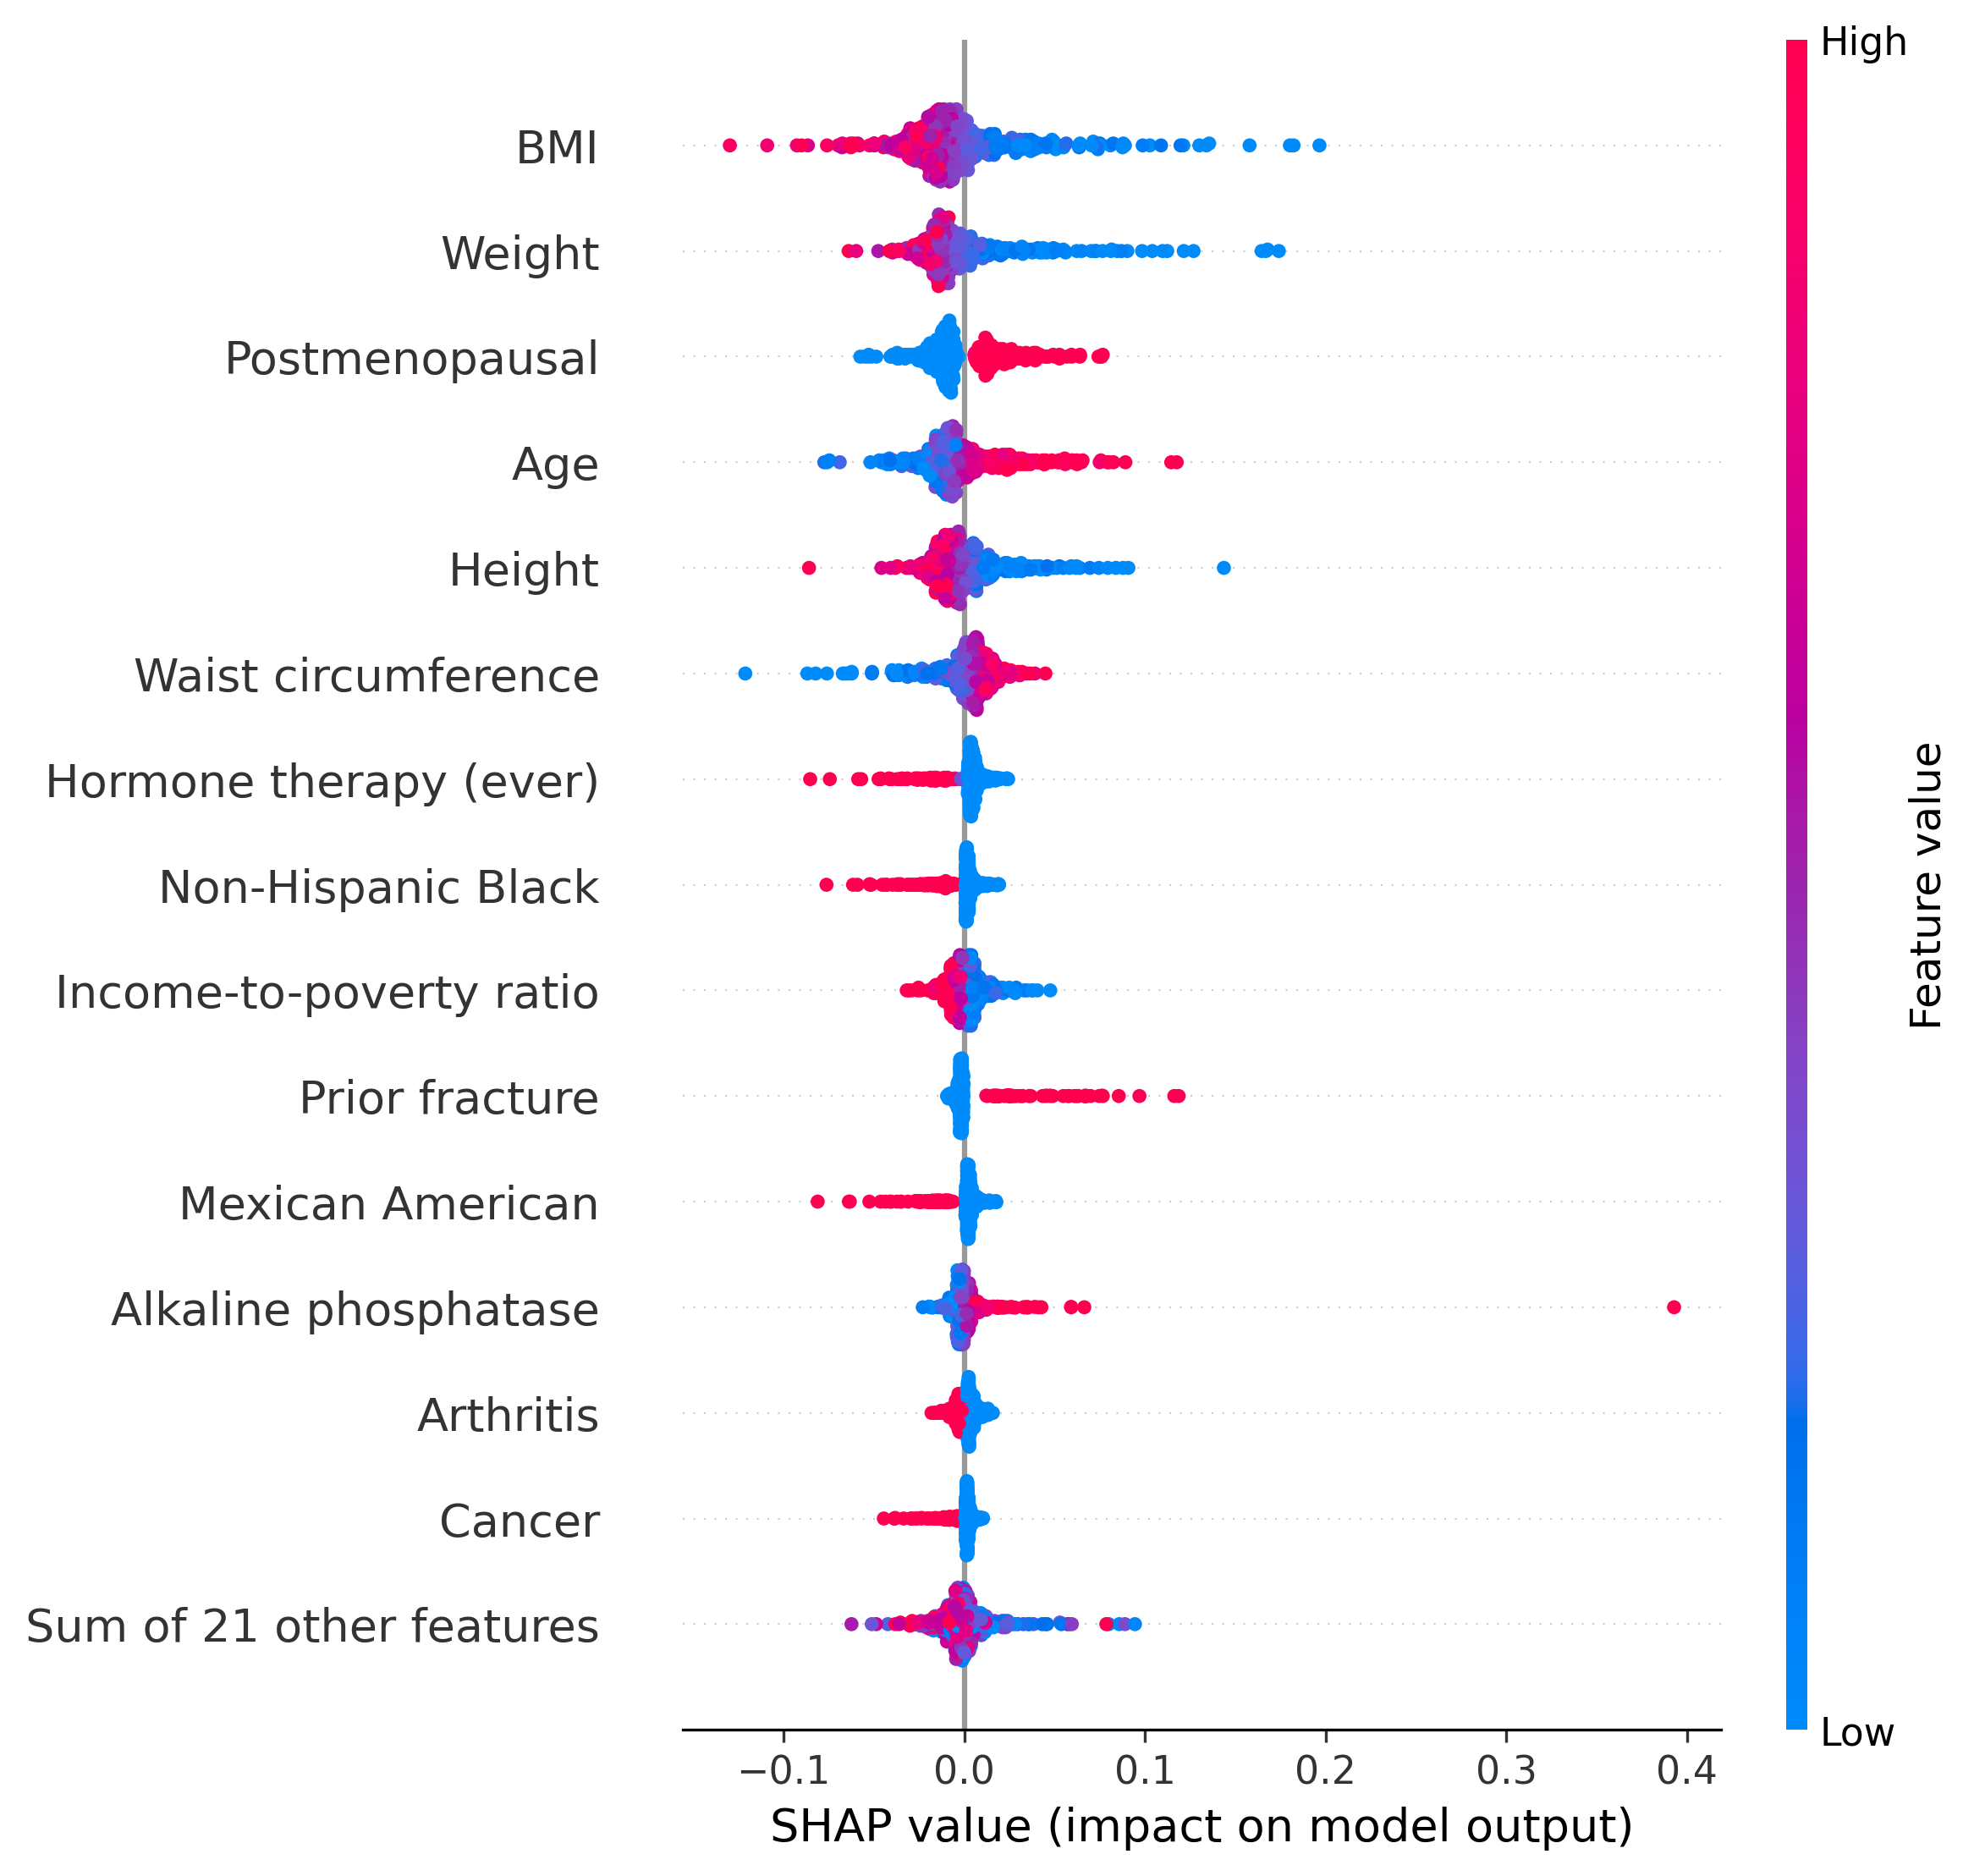
\includegraphics[width=0.64\textwidth]{fig6_shap_beeswarm.png}
\caption{SHAP beeswarm summary for the full model in 500 development-set participants (the sample used for importance ranking). Colour indicates the predictor value; horizontal position indicates its effect on predicted risk (probability scale, before recalibration).}
\label{fig:shap}
\end{figure}

\end{document}
